\chapter{Feature-based epipolar attention mechanism}
\label{chapter:epinerf}

\ifthenelse{\boolean{skipEpiNeRF}}{\endinput}{}


\section{Introduction}
Few-shot NVS presents a challenging task in computer vision, wherein the objective is to generate an image from an unobserved viewpoint using only a limited number of source images and their corresponding camera pose information. The present work addresses an even more intricate scenario, which exclusively relies on a unique source image. The problem is inherently ill-posed as a single source image may not provide enough visual clues to generate a novel viewpoint. Handling unforeseen elements as well as occlusions becomes particularly challenging in this scenario. To effectively tackle these challenges, leveraging 3D priors ~\citep{saito2019pifu,johari2022geonerf} is fundamental since it enables deep architectures to acquire a primary understanding of the underlying 3D scene structure. 

Recent advances in neural rendering significantly drive latest works in few shot NVS. While original neural radiance field (NeRF) ~\citep{mildenhall2020nerf} allows to represent a scene through a learned overfitted 5D function, it does not have any generalization abilities. Latest contributions ~\citep{yu2021pixelnerf,li2022symmnerf,lin2023vision} designed low-resolution 2D feature \textbf{F} conditioning to tackle such a limitation, mostly by leveraging on an image encoder. Produced feature volume is sampled at training and testing time through pixel-aligned bilinear interpolation to \textit{locally} condition the radiance field. However, the deep feature is aligned with the source view: occlusions and unobserved parts therefore lead to misaligned and coarsely-local feature on \textbf{F}, producing non-optimal conditioning. 

Our work therefore try to address such a limitation by producing target-aligned features from NeRFeature, a feature radiance field we designed. Associated training is supported through a light feature distillation procedure, by leveraging on a CNN encoder-decoder as teacher network. Target oriented feature (from the NeRFeature student radiance field) is then involved (with its source-aligned counterpart) in an epipolar-based attention mechanism: the weights sampling distribution is shrunk around regions where source and target features match. Our contributions are three-fold and can be summarised through: 
\begin{enumerate}
   \item A learned feature radiance field, called NeRFeature. Given a source-aligned feature and a camera transformation, NeRFeature aims to infer the correspond\--ing target-aligned deep feature trough a light feature distillation procedure, that do not involve any heavy foundation models (section \ref{subsec:nerfeature}). 
    \item A simple yet effective epipolar-based attention mechanism that relies on source and target aligned features and which adjust the weights sampling distribution during volume rendering (section \ref{subsec:epipolar_att}). 
    \item A novel generalizable NeRF architecture for single-image NVS, EpiNeRF, \textit{locally} conditioned on its input with a CNN as well as \textit{globally} conditioned on its weights through a Hypernetwork (section \ref{subsec:epinerf}).  
    
\end{enumerate}

\section{Related work}

\noindent\textbf{Single-image novel view synthesis.} Novel view synthesis aims to render an image of a scene from a an unobserved viewpoint, given a set of posed images, i.e. images and the associated camera poses (3D position and orientation). Synthesising a viewpoint from a different location based on a single image is an ill-posed task as occluded parts cannot be easily recovered in this scenario. While fully convolutional-based networks first appeared in the devoted literature ~\citep{kim2020novel,hou2021novel,guo2022fast,landreau2022epipolarnvs}, the emergence of neural radiance fields ~\citep{mildenhall2020nerf} highly influenced the way single-view novel view synthesis architectures ~\citep{yu2021pixelnerf,li2022symmnerf,lin2023vision} are built. Latest research directions in single-image NVS push toward extremely large deep networks, such as image-conditioned diffusion models ~\citep{chen2023single,gu2023nerfdiff,chan2023genvs}. Recent advances in foundational 3D reconstruction models  even explicitly grasp the whole 3D structure of an object from a single view ~\citep{liu2023zero,zou2023triplane}. However, these diffusion-based architectures remain complex to train and have poor speed inference performances.  

\noindent\textbf{Generalizable NeRF conditioning} Introduced in Mildenhall's \etal ~\citep{mildenhall2020nerf} work, a neural radiance field $\psi$ aims to implicitly represent the inherent geometry and appearance of a scene. In its original formulation, a set of posed images $\{I,\pi = K[R|t]\}$ is sufficient to learn such a radiance field.

However, above  formulation prevents the NeRF to generalise across multiple scenes. While plethora works nowadays rely on deep feature volume to condition their neural architecture ~\citep{wang2021ibrnet,chen2023matchnerf}, PixelNeRF ~\citep{yu2021pixelnerf} has paved the way to such limitation in single-image NVS. It locally conditions its radiance field using pixel-wise source aligned features, obtained from a CNN encoder-decoder. This \textit{local} -input based- conditioning is now commonly adopted in the devoted literature ~\citep{jang2021codenerf,li2022symmnerf,lin2023vision}.

\noindent\textbf{Feature distillation in NeRF.} A radiance field can be extended to output additional features of interest, and thus go beyond RGB space, as soon as a supervisory signal exists to train such an architecture.  Research from ~\citep{hinton2015distilling} paved the way for feature distillation, mostly to tackle both knowledge transfer and model compression issues. Few works already attempted to distill feature from a 2D model (such as a CNN or a ViT ~\citep{dosovitskiy2020vit}) into 3D through the use of neural radiance fields ~\citep{kobayashi2022decomposing}.  Whereas Jianglong Ye \etal ~\citep{ye2023featurenerf} learned a radiance field  by distilling feature from a 2D foundation model ~\citep{oquab2023dinov2}, we propose a lighter feature distillation procedure. 

\section{Method}
First subsection is devoted to the general NeRF formalism. We then present the different EpiNeRF sub-modules and how they have been trained. We present an overview of our architecture on Figure \ref{fig:overview}. 

\begin{figure}[htb!]
    \begin{center}
  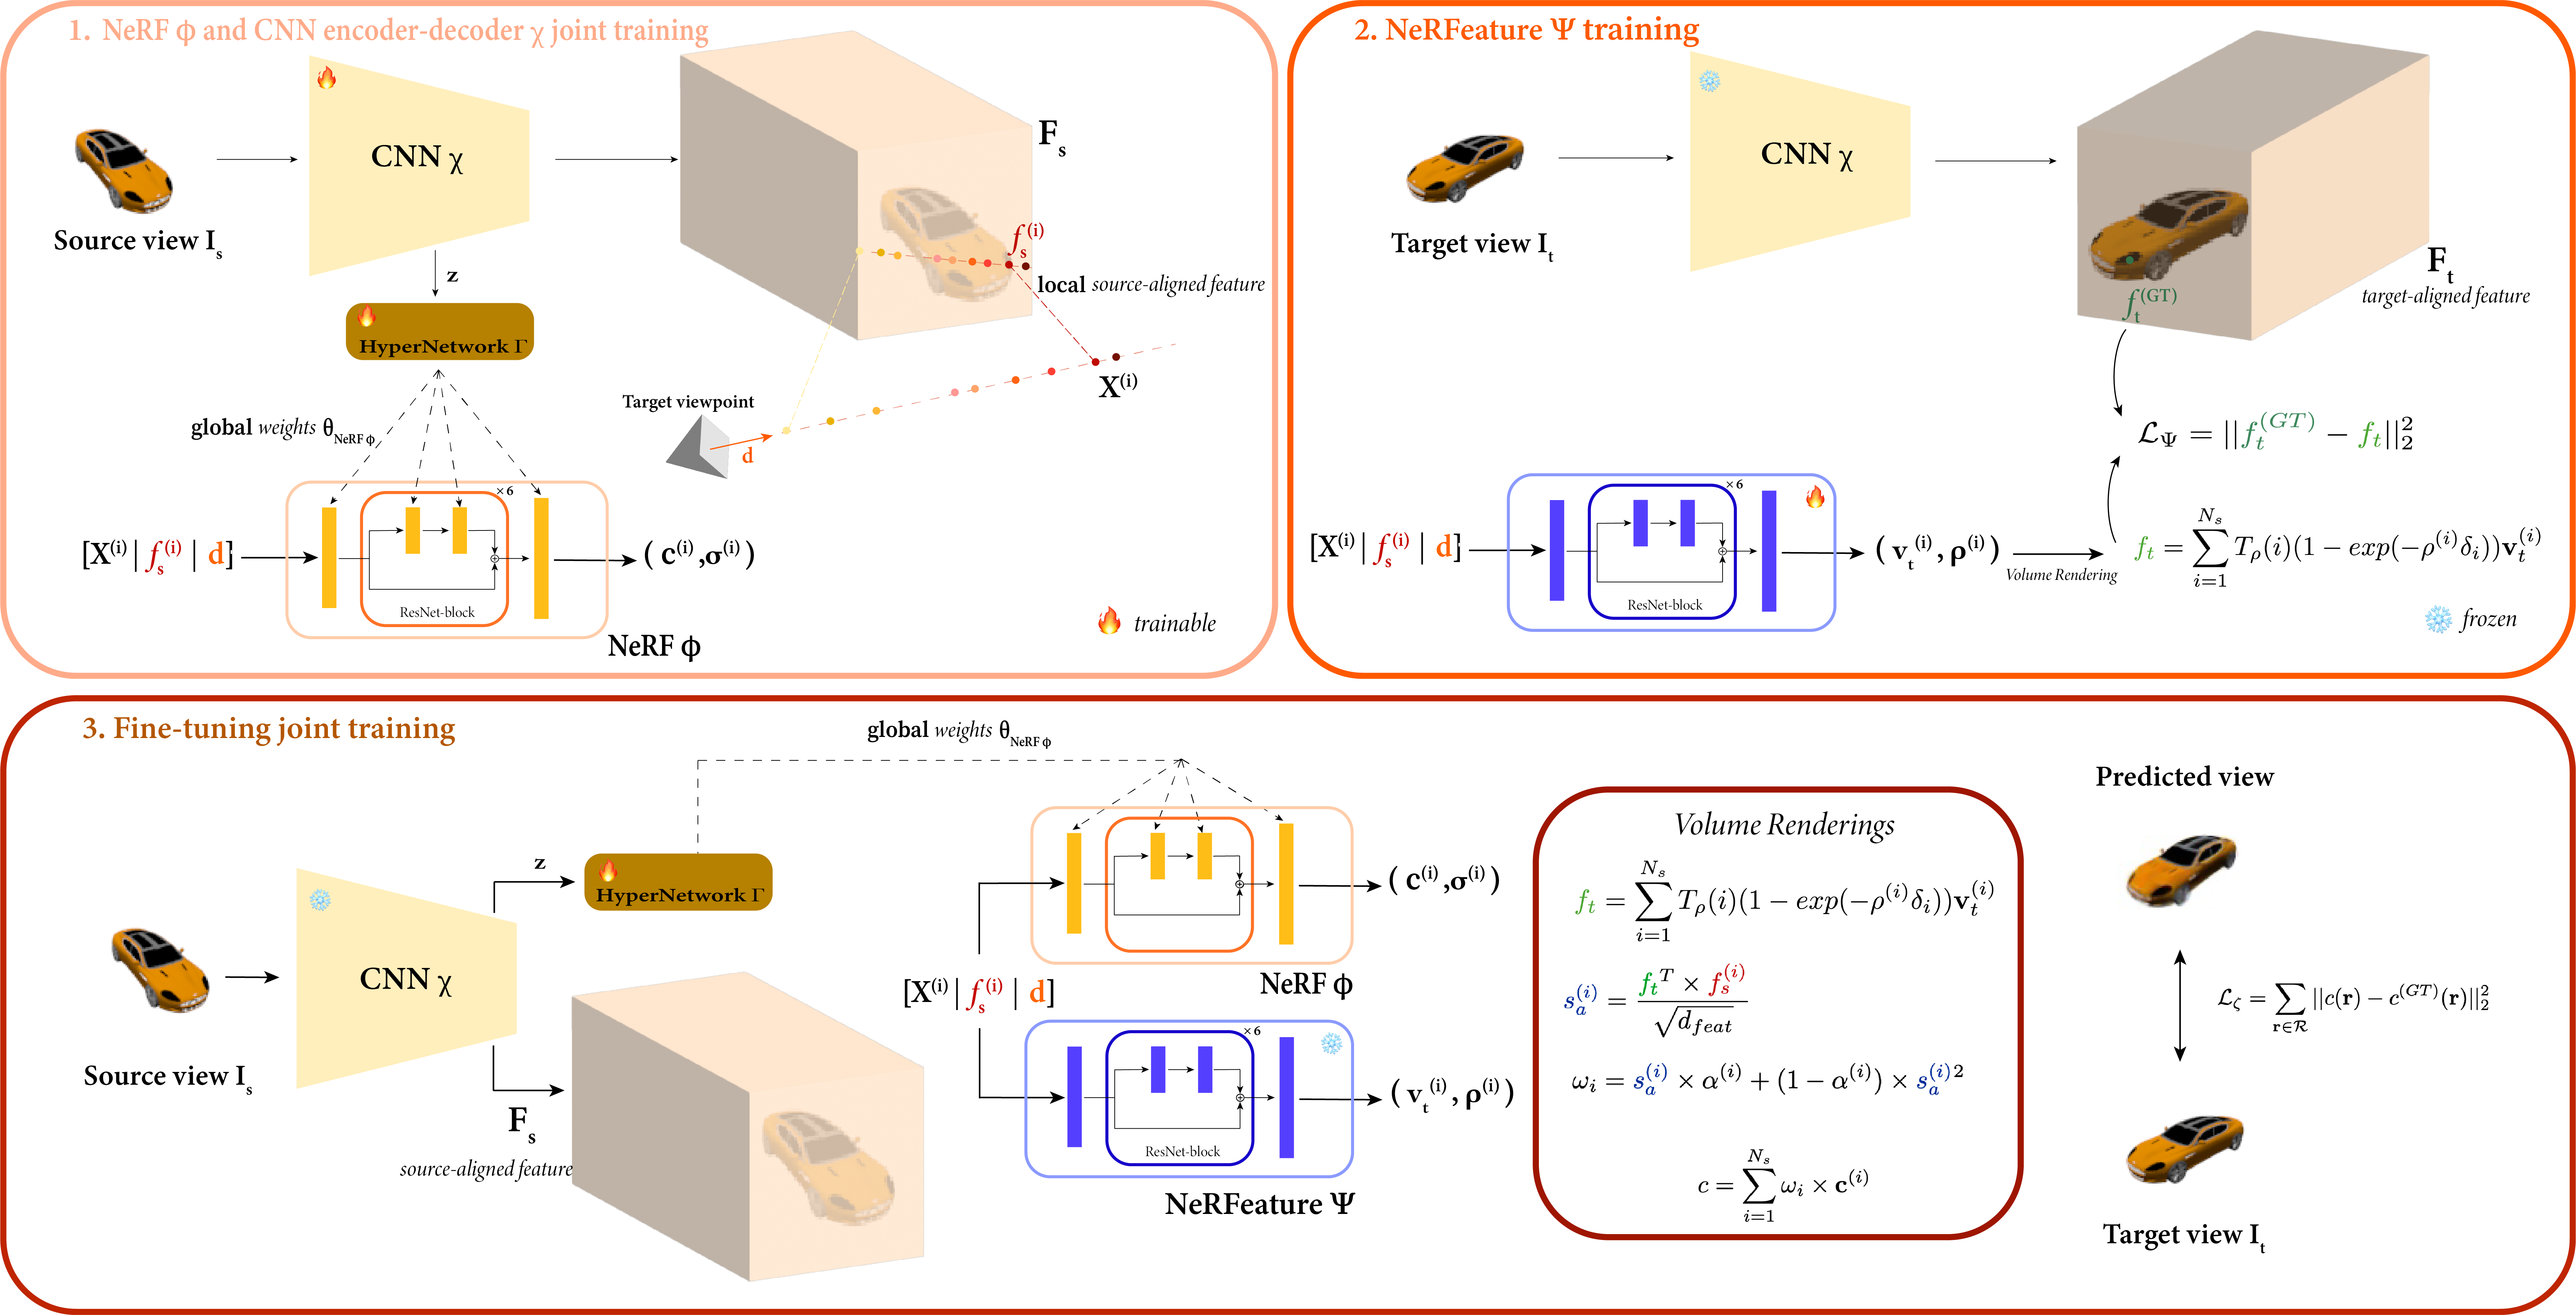
\includegraphics[width=\linewidth]{images/epinerf/overview_architecture.png}
  \end{center}
  \caption{\textbf{Overview of our complete three-stage training EpiNeRF architecture.} (Top left) The first step primarily aims to train our CNN encoder-decoder $\chi$. It generates \textit{local} features aligned with $I_{s}$. (Top right) CNN $\chi$ is used a teacher model to instruct a NeRF student model $\Psi$, termed NeRFeature, to generate deep features from any target viewpoint. (Bottom) Last training stage is a fine-tuning where our epipolar-based attention mechanism dynamically adjust the volume rendering equation through $\Psi$.}
  \label{fig:overview}
\end{figure}

\subsection{Background: NeRF}

Given a 3D point in world space $\mathbf{x} \in \mathbb{R}^{3}$ along a ray and its viewing direction $\mathbf{d} \in \mathbb{R}^{3}$, a vanilla RGB radiance field $\psi$ is entirely defined through its density $\sigma_{\psi}(\mathbf{x})\in \mathbb{R}_{+}$  and its RGB colour $c_{\psi}(\mathbf{x},\mathbf{d}) \in \mathbb{R}^{3}$. 
A differentiable volume rendering operation ~\citep{max1995optical} is performed to render the final composite RGB color $\hat{c}$ along the ray: 
\begin{equation}
\hat{c}  = \sum_{i}T_{\psi}^{(i)}\alpha_{\psi}^{(i)}c_{\psi}(\mathbf{x}^{(i)},\mathbf{d}) = \sum_{i} \omega_{\psi}^{(i)}c_{\psi}(\mathbf{x}^{(i)},\mathbf{d})
\end{equation}
with $\alpha_{\psi}^{(i)} = (1-\exp^{-\sigma_{\psi}(\mathbf{x}^{(i)})\delta_{i}})$ Term $\delta_{i} = \mathbf{x}^{(i+1)} - \mathbf{x}^{(i)} $ refers to the distance between two consecutive samples along the ray.

Field $\alpha_{\psi}$ should be interpreted as the probability of hitting a particle during an infinitesimal distance\footnote{Discretize through the term $\delta_{i} = x^{(i+1)} - x^{(i)}$} travel  along the ray $\mathbf{r}$. Term $ 1 - \alpha_{\psi}$ thus illustrates the probability of not hitting any particle over such a displacement. 

Transmittance $T_{\psi}^{(i)} = \prod_{j=1}^{i}(1-\alpha_{\psi}^{(j)})$ has to be considered as the probability, over the interval $[x_{near},x^{(i)})$, to not hit any particles while travelling along $\mathbf{r}$. We define $x_{near}$ as the very first point sampled along a ray $\mathbf{r}$. Such a transmittance term can also be easily refactored as: 
\begin{equation}
T_{\psi}^{(i)} = \exp\left( - \sum_{j=1}^{i}\sigma_{\psi}^{j}\delta_{j}\right)
\end{equation}

Term $T_{\psi}^{(i)}\alpha_{\psi}^{(i)}$ in the final composite RGB color $\hat{c}$ should therefore be interpreted as the likelihood that ray terminates exactly at index $i$.  We now omit network indexing over these variables for clarity purpose.

\subsection{NeRFeature: learn target-aligned features}
\label{subsec:nerfeature}

While feature volumes produced by any 2D models (CNN or ViT) are defacto aligned with the RGB image they have been fed with (i.e the source image $I_s$), we propose to distil the feature space into 3D through a neural feature radiance field, termed NeRFeature $\Psi$. 

NeRFeature inner architecture is depicted on Figure \ref{fig:supp_nerfeature}. It follows quite closely the radiance structure of $\Phi$, even though there is no hypernetwork involved here to predict $\Psi$ weights. NeRFeature aims to produce deep features that lives in the learned latent space from $\chi$, similarly to what \cite{ye2023featurenerf} implemented by distilling foundation models \cite{oquab2023dinov2}.

\begin{figure}[h!]
    \begin{center}
  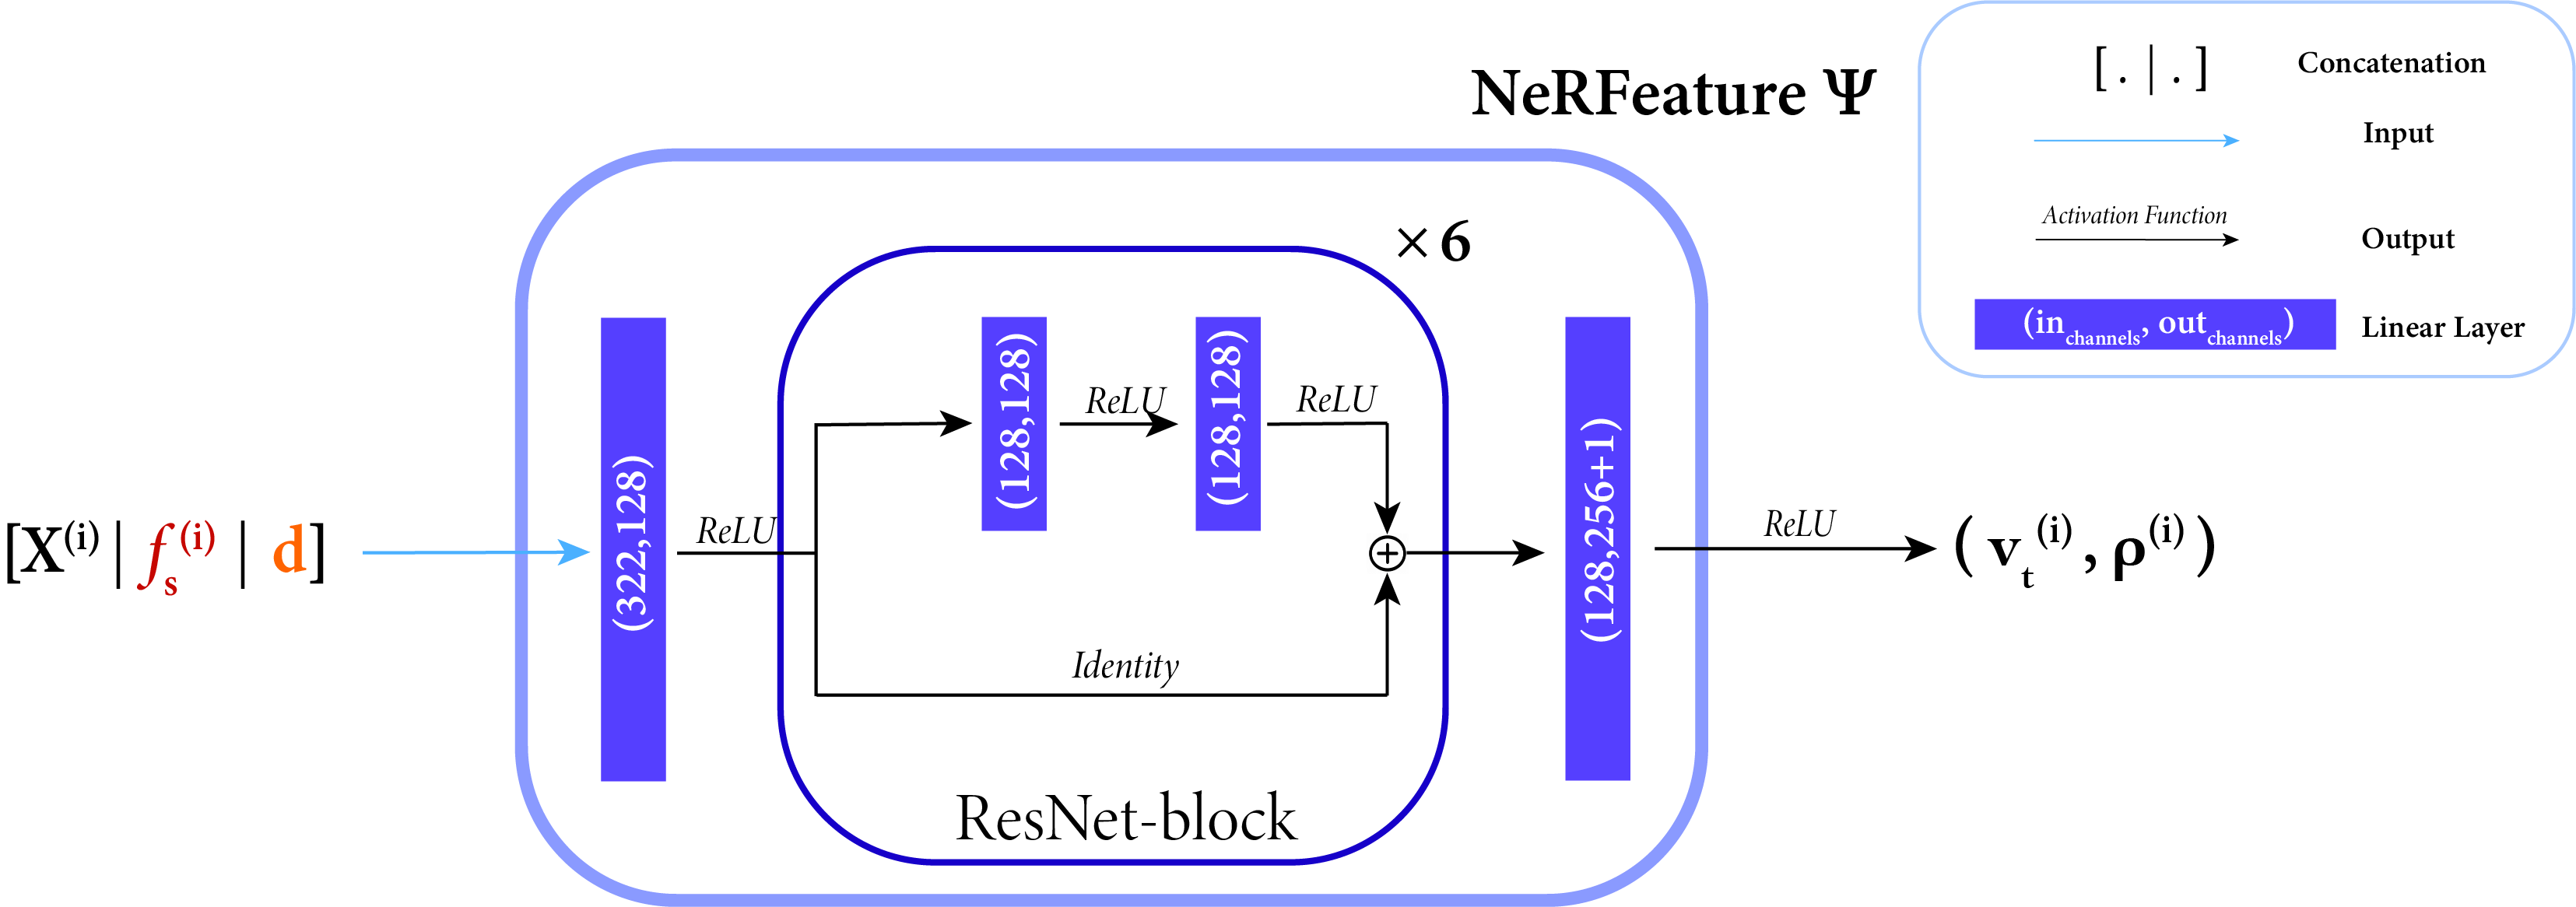
\includegraphics[width=\linewidth]{images/epinerf/supp_nerfeature.png}
  \caption{NeRFeature implements a six ResNet blocks inner architecture, but with an extended output, that lives in $\mathbb{R}^{d_{\text{feat}}}$. Such an intermediate dense feature, well as a transparency scalar, that are later involved in the volume rendering operation to get $f_{t}$. }
  \label{fig:supp_nerfeature}
  \end{center}
\end{figure}


A pretrained teacher 2D CNN encoder $\chi$ (top-left panel on Figure \ref{fig:overview}) produces \textit{pseudo} ground truth features, that are used to supervise the training distillation of the NeRFeature $\Psi$ (top-right panel on Figure \ref{fig:overview}).

Given any 3D point $\mathbf{x}^{(i)}$ expressed in the world coordinate system along a ray $\mathbf{r}$ from a target direction $\mathbf{d}$, we denote: 

\begin{equation}
    f_{s}^{(i)} = \mathbf{F}_{s}(\pi(\mathbf{x}^{(i)}))  \in \mathbb{R}^{d_{\text{feat}}} 
    \label{eq:projection}
\end{equation}

the source-aligned feature that was extracted from $\mathbf{F}_{s}=\chi(I_{s})$ through the perspective projection $\pi$ of $\mathbf{x}^{(i)}$ on the feature plane.

As $\Psi$ must be generalizable (\textit{i.e} render meaningful features for unseen objects or scene), NeRFeature has to be conditioned with $f_{s}^{(i)}$: 

\begin{equation}
    \Psi(\mathbf{x}^{(i)},\mathbf{d},f_{s}^{(i)}) = (\rho^{(i)},\mathbf{v}_{t}^{(i)}) \in \mathbb{R}_{+}\times \mathbb{R}^{d_{\text{feat}}}
\end{equation}

while the target-aligned feature $\mathbf{f}_{t}$ is obtained through the vanilla volume rendering equation computed over the $N_s$ sampled points on \textbf{r}: 

\begin{equation}
    f_{t} = \sum_{i=1}^{N_{s}} T_{\rho}^{(i)}(1-exp(-\rho^{(i)}\delta_{i}))\mathbf{v}_{t}^{(i)}
\end{equation}

with $\delta_{i}=\mathbf{x}^{(i+1)}-\mathbf{x}^{(i)}$  the distance between two consecutive samples and $T_{\rho}^{(i)} = \exp\left(-\sum_{j=1}^{i}\rho^{(j)}\delta_{j}\right)$ the accumulated transmittance along \textbf{r}.

As observed on Figure \ref{fig:supp_nerfeature}, symmetrical pixel-wise feature $f_{s,symm}^{(i)}$ is not provided as input to NeRFeature $\Psi$, as trying to integrate 3D symmetry prior in such a high dimensional space as $\mathbb{R}^{d_{\text{feat}}}$ would not be as easy as in the RGB space of $\Phi$. Only 3D point location, direction and the source-aligned feature $f_{s}^{(i)}$ are fed as input to NeRFeature. 

 Such a learned feature field is finally queried (see Section \ref{subsec:epipolar_att}) during the fine-tuning (Figure \ref{fig:overview} - bottom) phase to render the target-aligned features involved in our epipolar-based attention mechanism. 
 
\subsection{Feature-based epipolar attention}
\label{subsec:epipolar_att}

We extensively present in this section the entire feature-attention based mechanism we implemented in our EpiNeRF architecture. An overview is shown on Figure \ref{fig:attention_overview}. 

\begin{figure}[h!]
    \begin{center}
  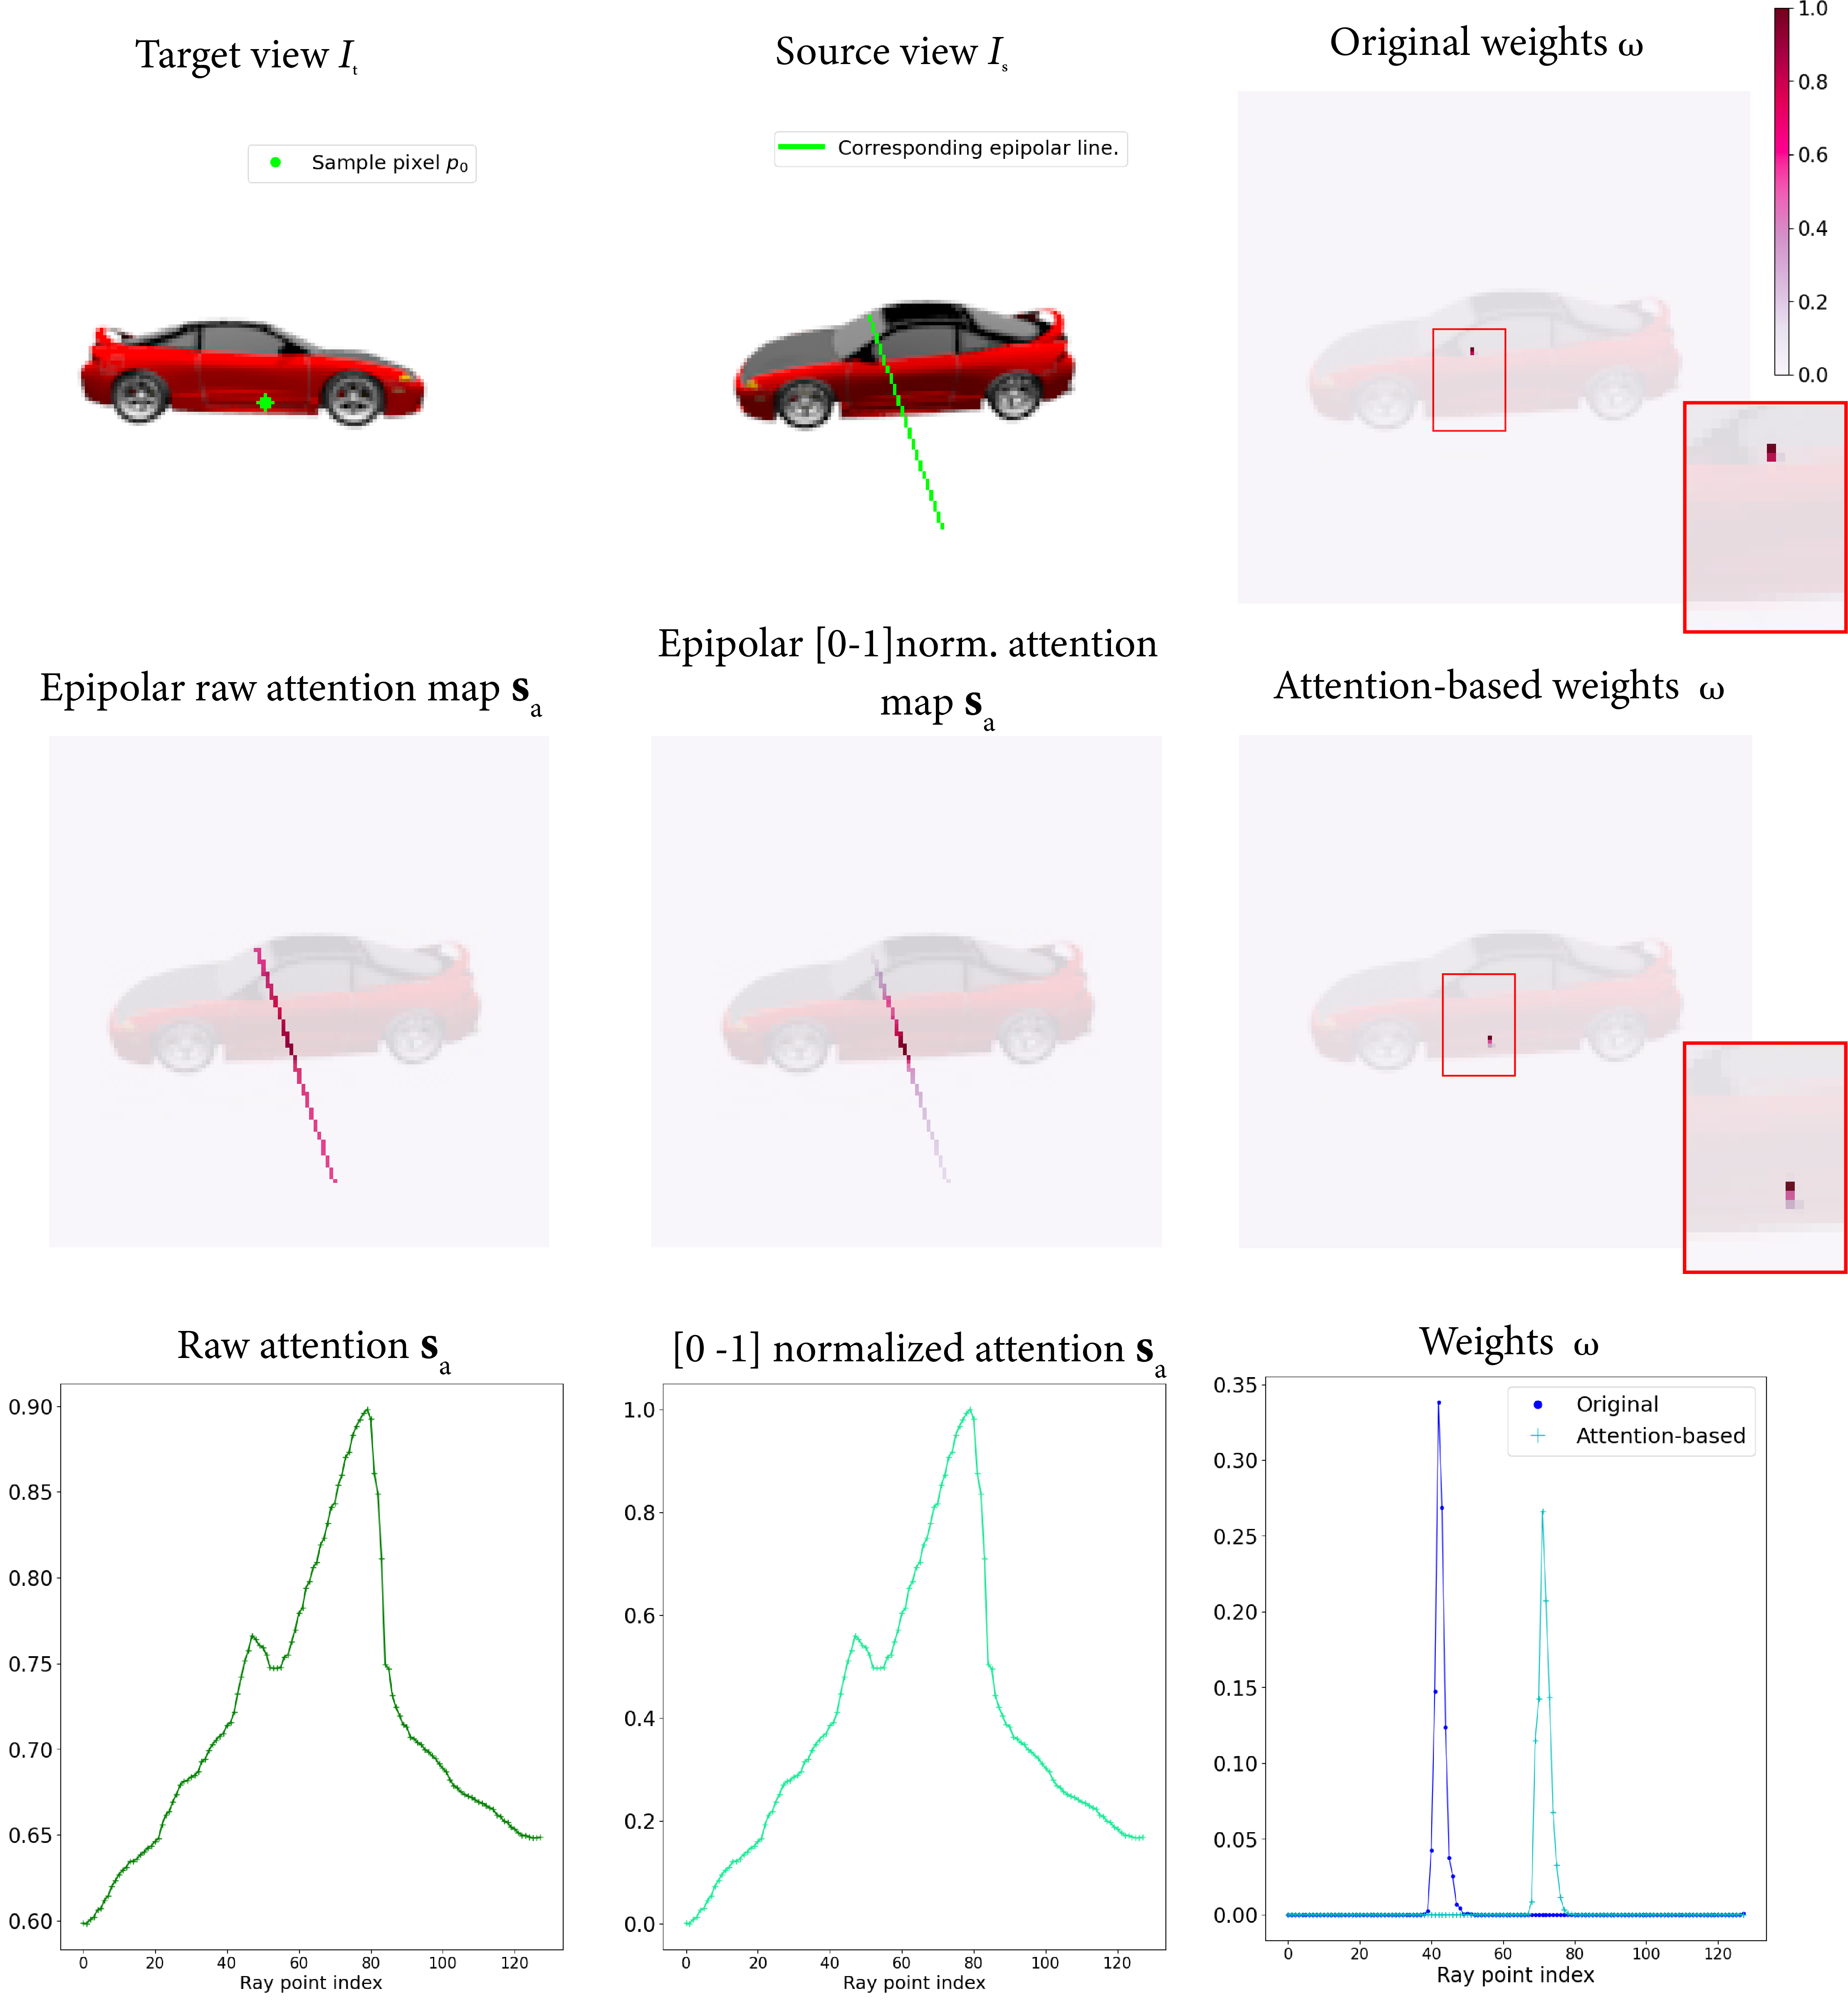
\includegraphics[width=\linewidth]{images/epinerf/SUPP_COMPLETE_OVERVIEW_OVERLEAF.png}
  \caption{Complete overview of our feature-based attention mechanism. Starting point of this study is the $p_{0}$ sampled pixel on the target viewpoint $I_{t}$. Associated epipolar line is shown on the source view $I_{s}$. }
  \label{fig:attention_overview}
  \end{center}
\end{figure}

Target-aligned features that are learn through $\chi$ knowledge distillation in $\Psi$ are used to compute a lightweight cross-attention like distribution ~\citep{vaswani2017attention} with the original source-aligned features. Indeed, $\Psi$ prediction $\mathbf{f}_{t}$ (\textit{key} \textbf{k}) and the source-aligned features $\mathbf{f}_{s}^{(i)}$(\textit{queries} \textbf{q}) that all lie on the epipolar line defined by the sampled pixel on the target view define a cross-attention $\mathbf{s}_{a}^{(i)}$:

\begin{equation}
    s_{a}^{(i)} = \frac{\mathbf{q}^{T}\mathbf{k}}{\sqrt{d_{\text{feat}}}}= \frac{f_{t}^{T}\times f_{s}^{(i)}}{\sqrt{d_{\text{feat}}}}
\label{eq:attention}
\end{equation}

while $\mathbf{s}_{a}=\{s_{a}^{(i)}\}_{i=1}^{N_{s}}$ denotes the entire distribution over the $N_s$ samples drawn along the ray $\mathbf{r}$. Both the raw and [0-1] normalized cross-attention distribution $\mathbf{s}_{a}$ are displayed either as epipolar attention maps (\textit{middle} row on first and second columns of Figure \ref{fig:attention_overview}) or a 1-dimensional distribution (\textit{last} row on first and second columns of Figure \ref{fig:attention_overview}). \newline

However, such a cross-attention distribution $\mathbf{s}_{a}$ can hardly be used as-is in the volume rendering equation. Indeed,  those distributions are not sharp enough to have the influence we aim at on the volume rendering equation. We thus need to shrink the normalized $\mathbf{s}_{a}$  distribution in a differentiable way around its maxima to obtain $\hat{\mathbf{s}_{a}}$. 

We thus designed two scaled sigmoid functions, called $S^{k}$ and $S^{K}$. 

\begin{align}
\hat{\textbf{s}}_{a} &= S^{K}(\textbf{s}_{a})\times S^{k}(\textbf{s}_{a}) \\
S^{q}(\mathbf{s}_{a}) &= \left(1- e^{q(\mathbf{s}_{a}-a_{0})}\right)^{-1}
\end{align}

while $q$ controls the sigmoid slope strength. Term $a_{0}$ allows to shift the sigmoid mid-value \textit{0.5} from 0 to $a_{0}$. Figure \ref{fig:attention_sigmoid} reflects these equations.

\begin{figure}[h!]
    \begin{center}
  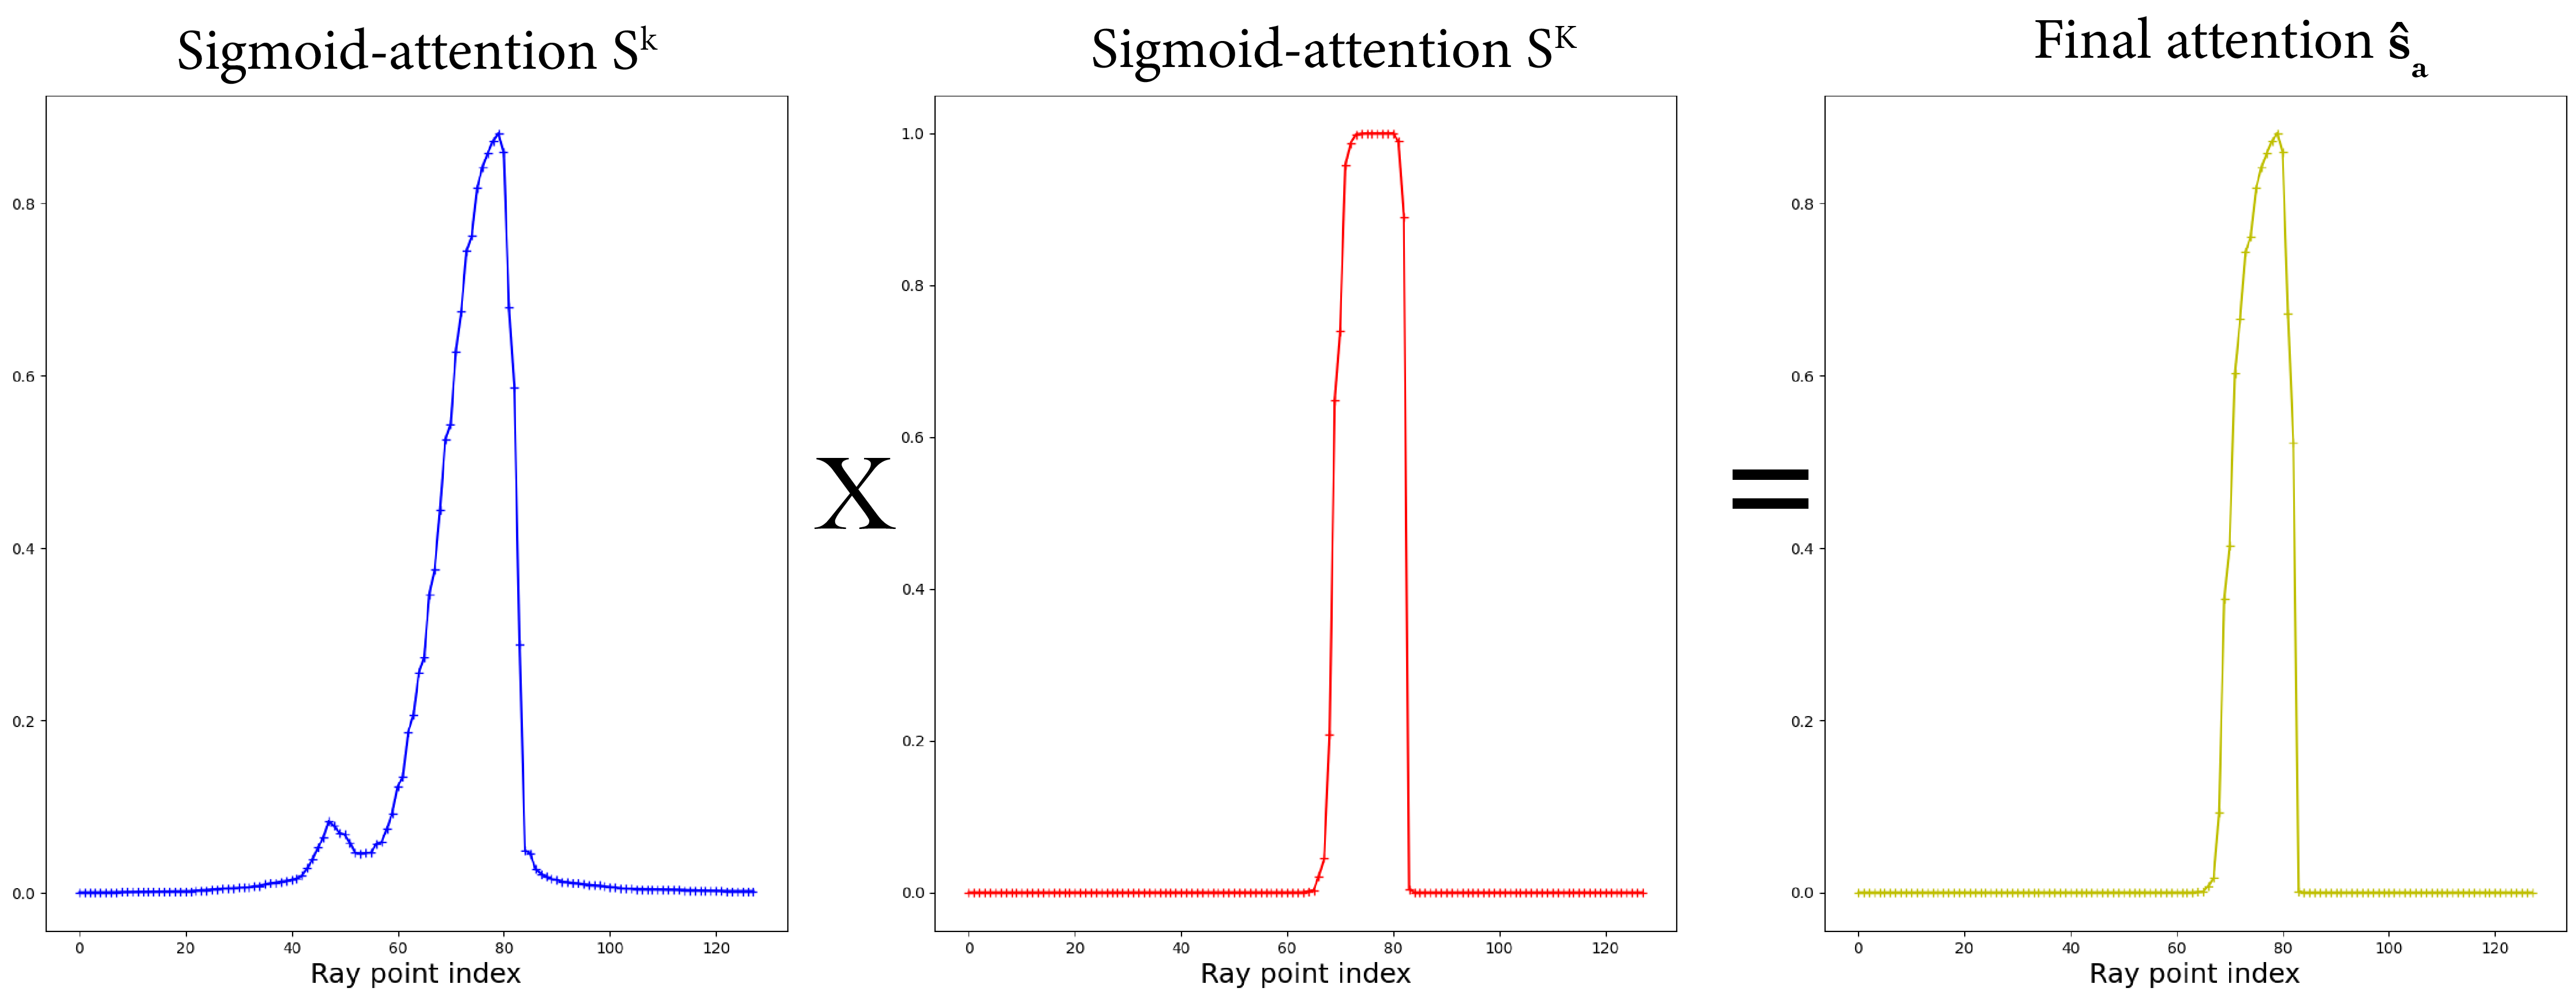
\includegraphics[width=\linewidth]{images/epinerf/SUPP_ATT_OVERLEAF.png}
  \caption{Intermediate attention distributions $S^{k}$ (\textit{left}) and $S^{K}$ (\textit{center}) allow to get $\hat{\mathbf{s}_{a}}$ (\textit{right}), the final attention distribution involved in the EpiNeRF architecture.}
  \label{fig:attention_sigmoid}
  \end{center}
\end{figure}

Setting such an hyperparameter to a non-null value allow to push attention scores that are lower than  $a_{0}$ toward 0.0 while attention that are higher than $a_{0}$ are thus drived against the maximum attention set to 1. We empirically set $k=10$, $K=60$ and $a_{0}=0.8$ during the EpiNeRF fine-tuning stage. \newline

This normalized and sigmoid-adjusted $\hat{\textbf{s}}_{a}$ attention distribution is then directly involved into the rendering process through the $\alpha$ blending we designed: 

\begin{equation}
\alpha  \gets \hat{\textbf{s}}_{a}\alpha + (1-\alpha)\hat{\textbf{s}}_{a}^{2}
\end{equation}

We illustrate such a blending operation on Figure \ref{fig:attention_construction}. 

\begin{figure}[h!]
    \begin{center}
  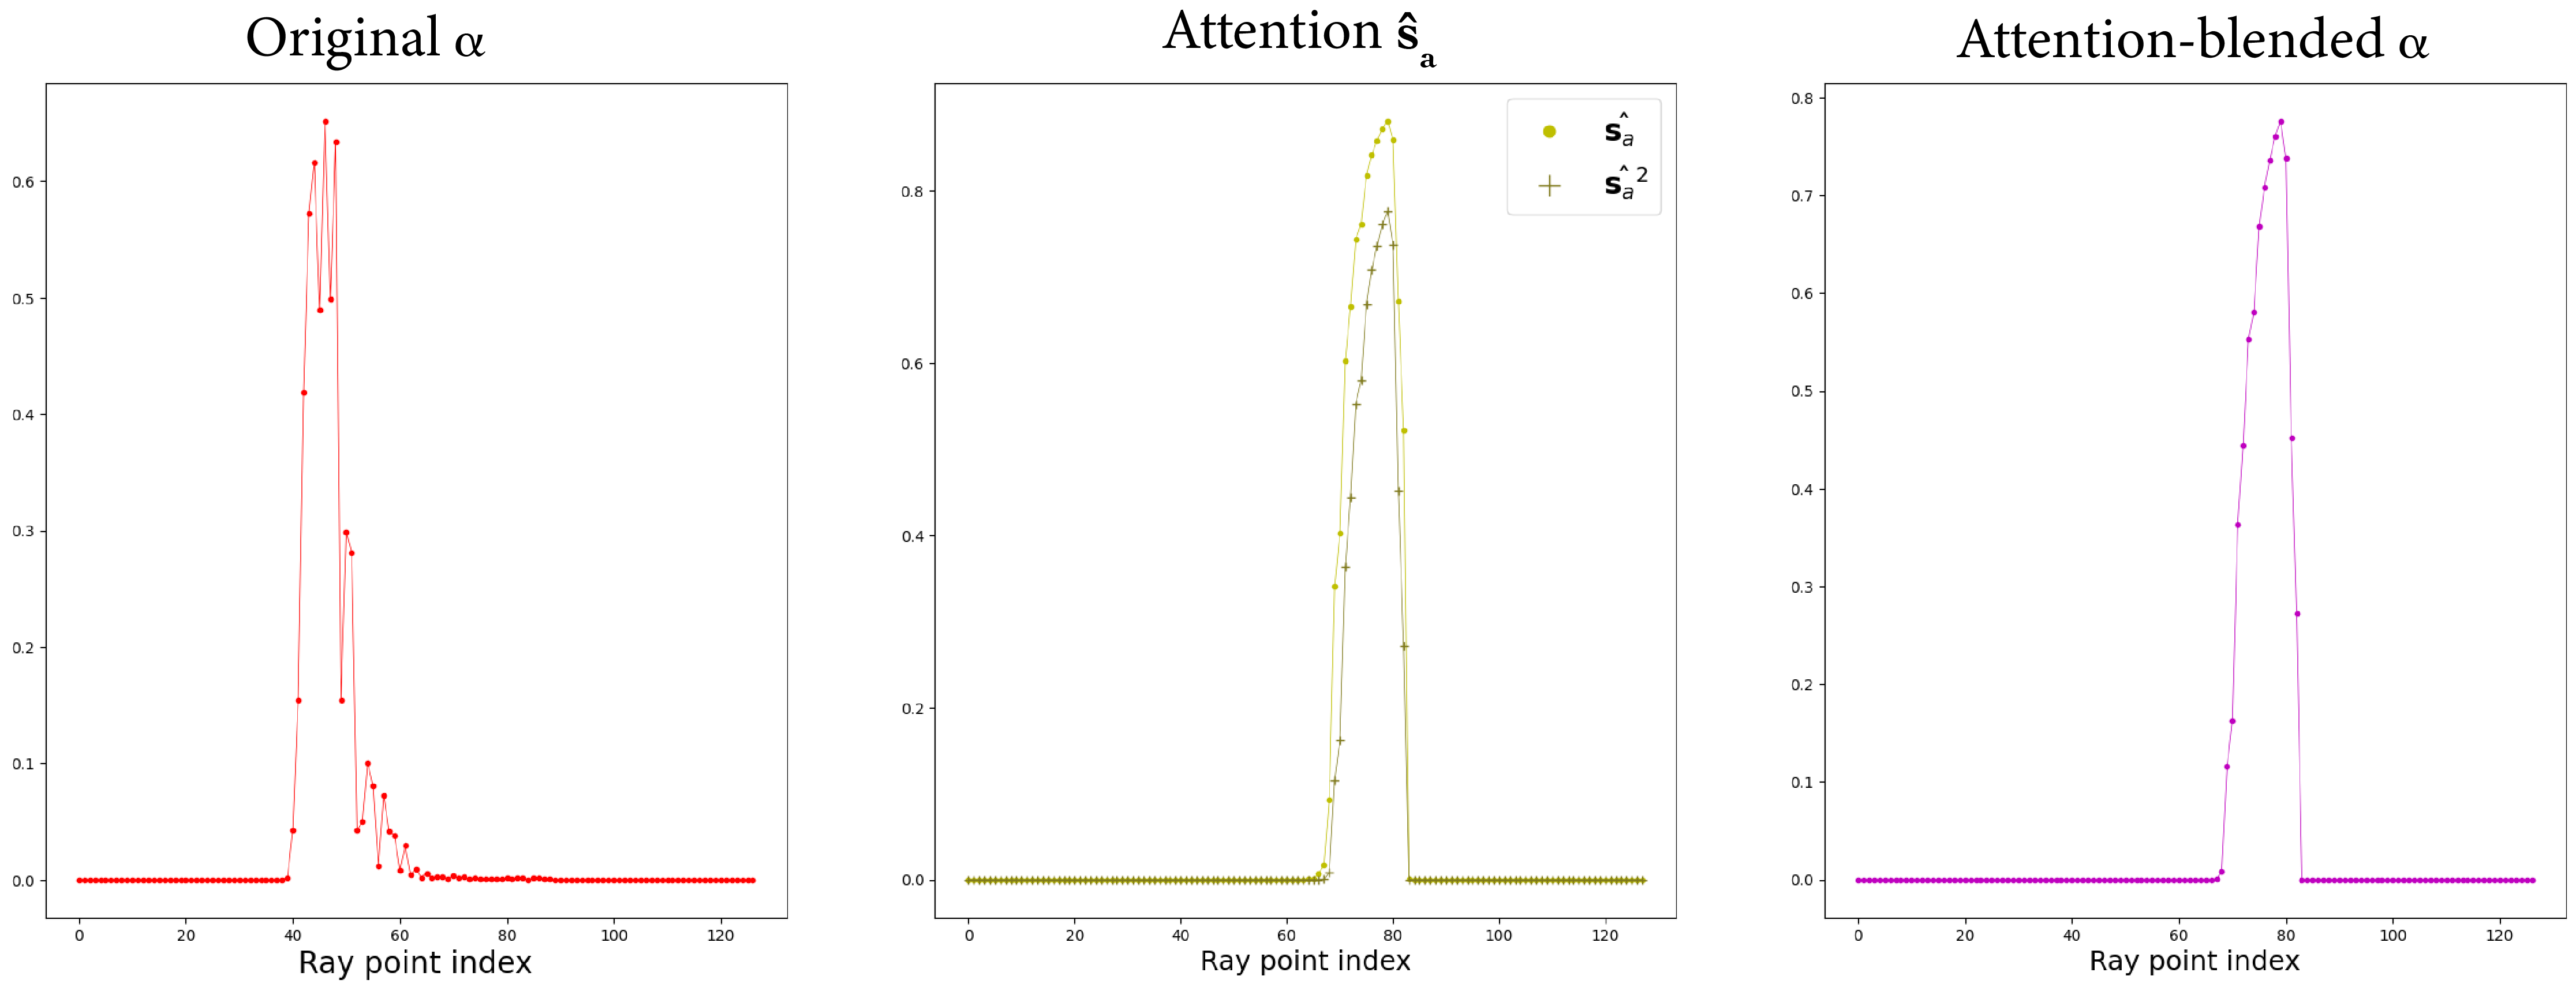
\includegraphics[width=\linewidth]{images/epinerf/SUPP_BLENDED_OVERLEAF.png}
  \caption{Illustration of the $\alpha$ attention-based blending correction. Original $\alpha$ distribution (\textit{left}) and its corrected attention-based counterpart (\textit{right}) show different activation regions along the ray. Attention distributions $\hat{\textbf{s}}_{a}$ and $\hat{\textbf{s}}_{a}^{2}$ are plotted in the \textit{center} panel.}
  \label{fig:attention_construction}
  \end{center}
\end{figure}

\begin{figure}[h!]
    \begin{center}
  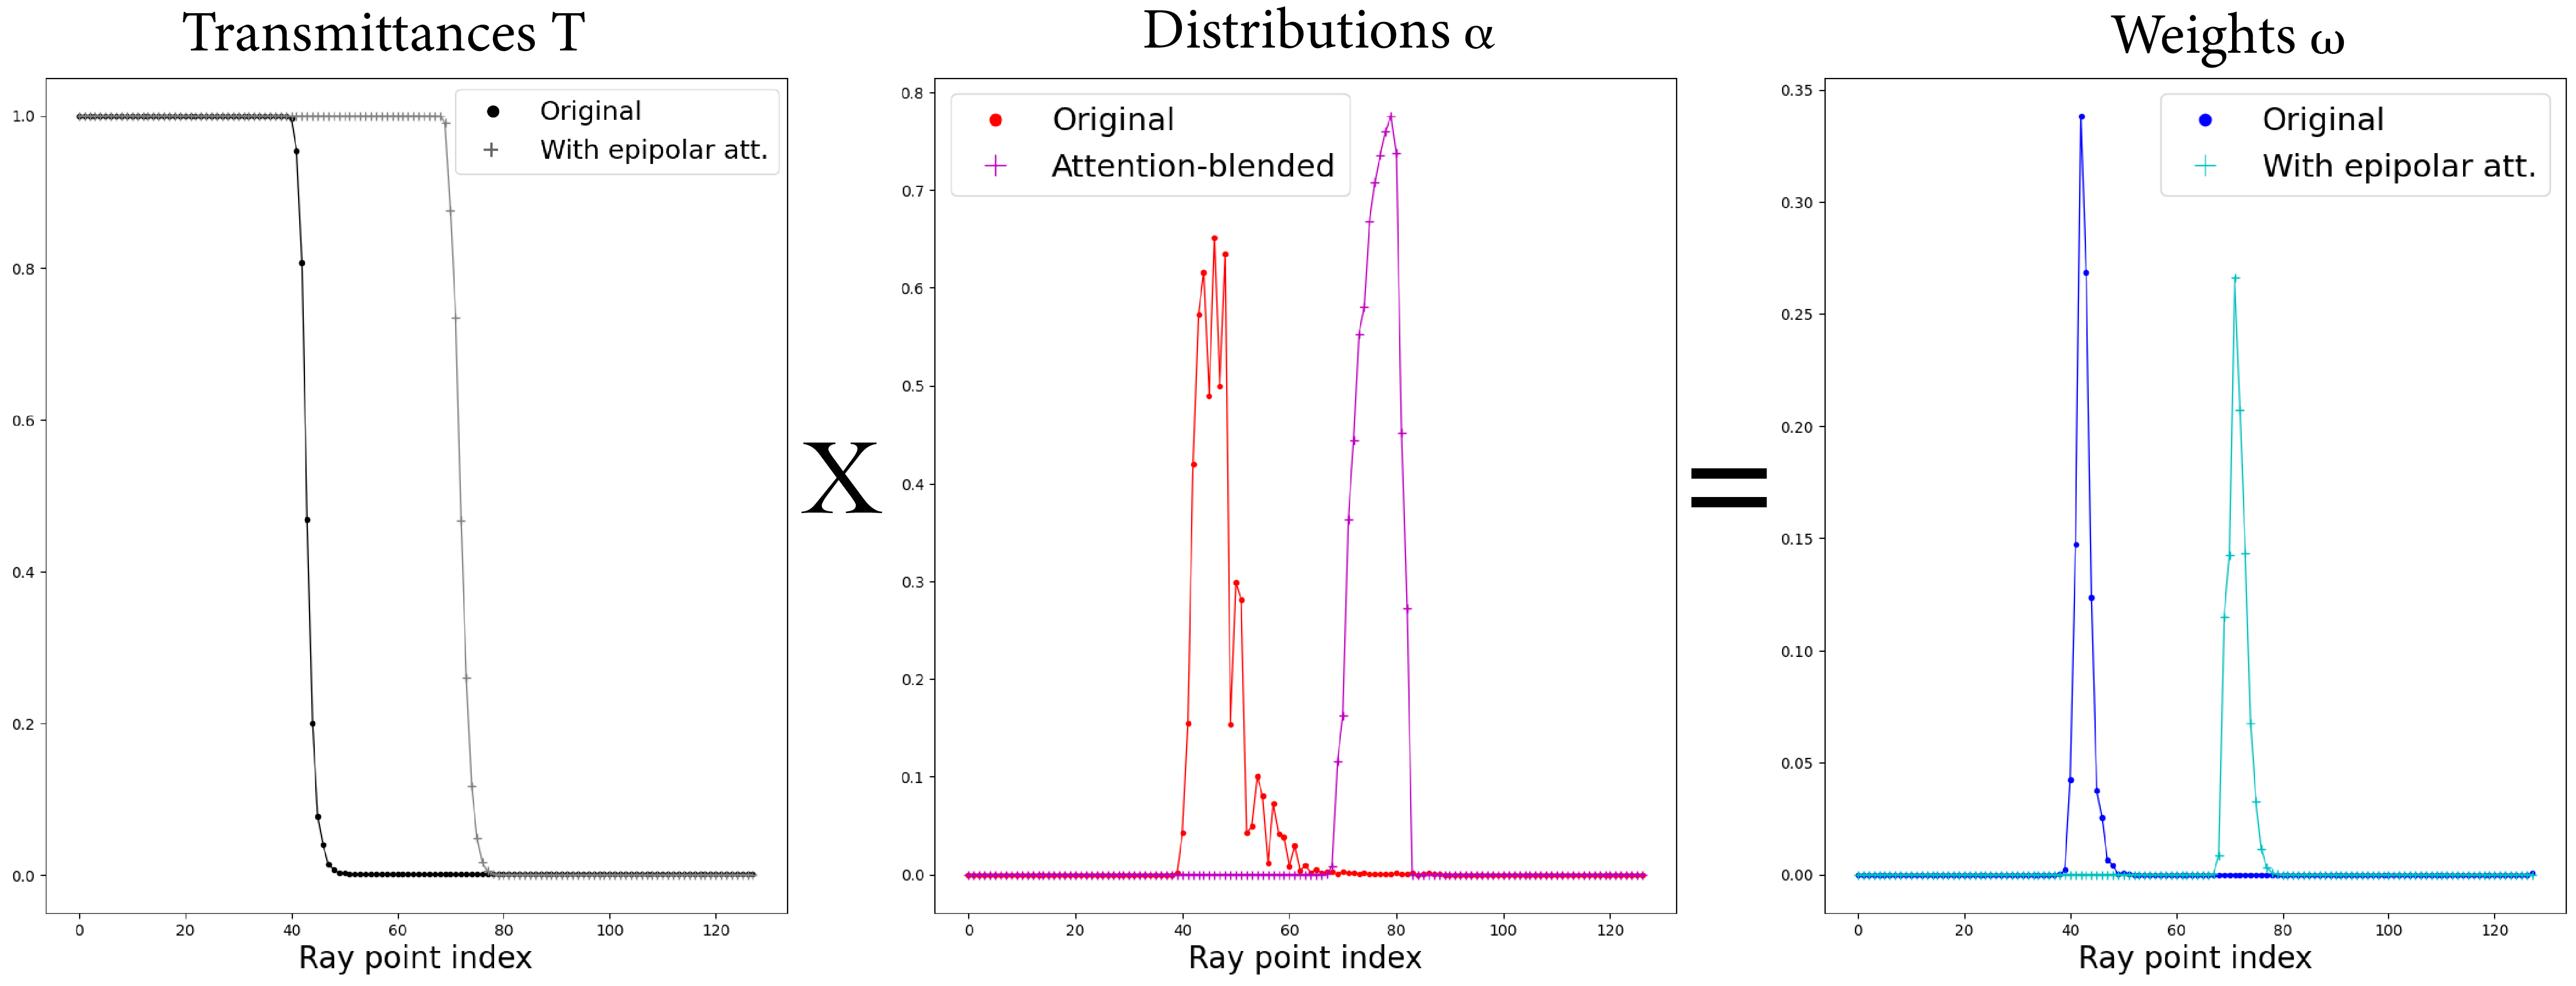
\includegraphics[width=\linewidth]{images/epinerf/SUPP_VR_OVERLEAF.png}
  \caption{Influence of our epipolar attention mechanism over the volume rendering equation. }
  \label{fig:overall_attention}
  \end{center}
\end{figure}

This attention-based correction over the $\alpha$ has finally a direct influence on the transmittance \textbf{T} as soon as it is the cumulative product of the $1-\alpha^{(i)}$ terms. We observe on Figure \ref{fig:overall_attention} how both transmittance and $\alpha$ distribution shift the final weight distribution toward region were attention $\hat{\textbf{s}}_{a}$  reaches its maximal values. As attention-corrected $\alpha$ distribution is shifted toward higher indexes along $\mathbf{r}$ (where attention is maximal), the corresponding transmittance is thus affected in a similar manner. Our epipolar attention module therefore stresses on the need for the ray to terminate later ($\sim$ \textit{index} $80^{th}$), contrary to the initial predictions ($\sim$ \textit{index} $50^{th}$). \newline 

First two rows of Figure \ref{fig:attention_overview} last column finally exhibits where meaningful weights have been put in the source domain. Our feature cross-attention module tries to focus on source view regions that semantically match with the pixel that was sampled on the target viewpoint(\textit{i.e} on the bottom of the door rather than on the window) even if such a region is unobserved in $I_s$.

Beyond correcting the volume rendering equation, our attention mechanism also allows to sample better and more relevant 3D points for $\Phi$ fine-NeRF prediction.

As soon as deep features from $\chi$ has been distilled into the NeRFeature $\Psi$, target-aligned features can be synthesized by solely requiring the source-aligned feature and a ray to sample.



\subsection{EpiNeRF: the complete architecture}
\label{subsec:epinerf}
\noindent\textbf{CNN-based source-aligned features.} Plethora of recent NeRF-based NVS works leverage their radiance field on a source-aligned feature volume $\mathbf{F}_{s}$, obtained from either a CNN ~\citep{jang2021codenerf,yu2021pixelnerf,li2022symmnerf} or a ViT ~\citep{lin2023vision}. However, intermediate features produced by the inner encoder are often fused and upscaled in a vanilla way, through bilinear upsampling and concatenation in the CNN decoder. 
Such a source-aligned feature volume can be built differently, by accounting on residual connections and atrous convolutions, as ~\citep{chan2023genvs} did too. 
EpiNeRF thus rather gets consideration for DeepLabV3+ ~\citep{chen2018encoder} backbone decoder to produce $\textbf{F}_{s}\in \mathbb{R}^{d_{\text{feat}} \times H \times W}$. It therefore has the same resolution as the input image $\mathbf{I}_s$. An overview of these two different feature fusion strategies is depicted on Figure \ref{fig:feature_encoder}. 

\begin{figure*}[h!]
  \begin{center}
  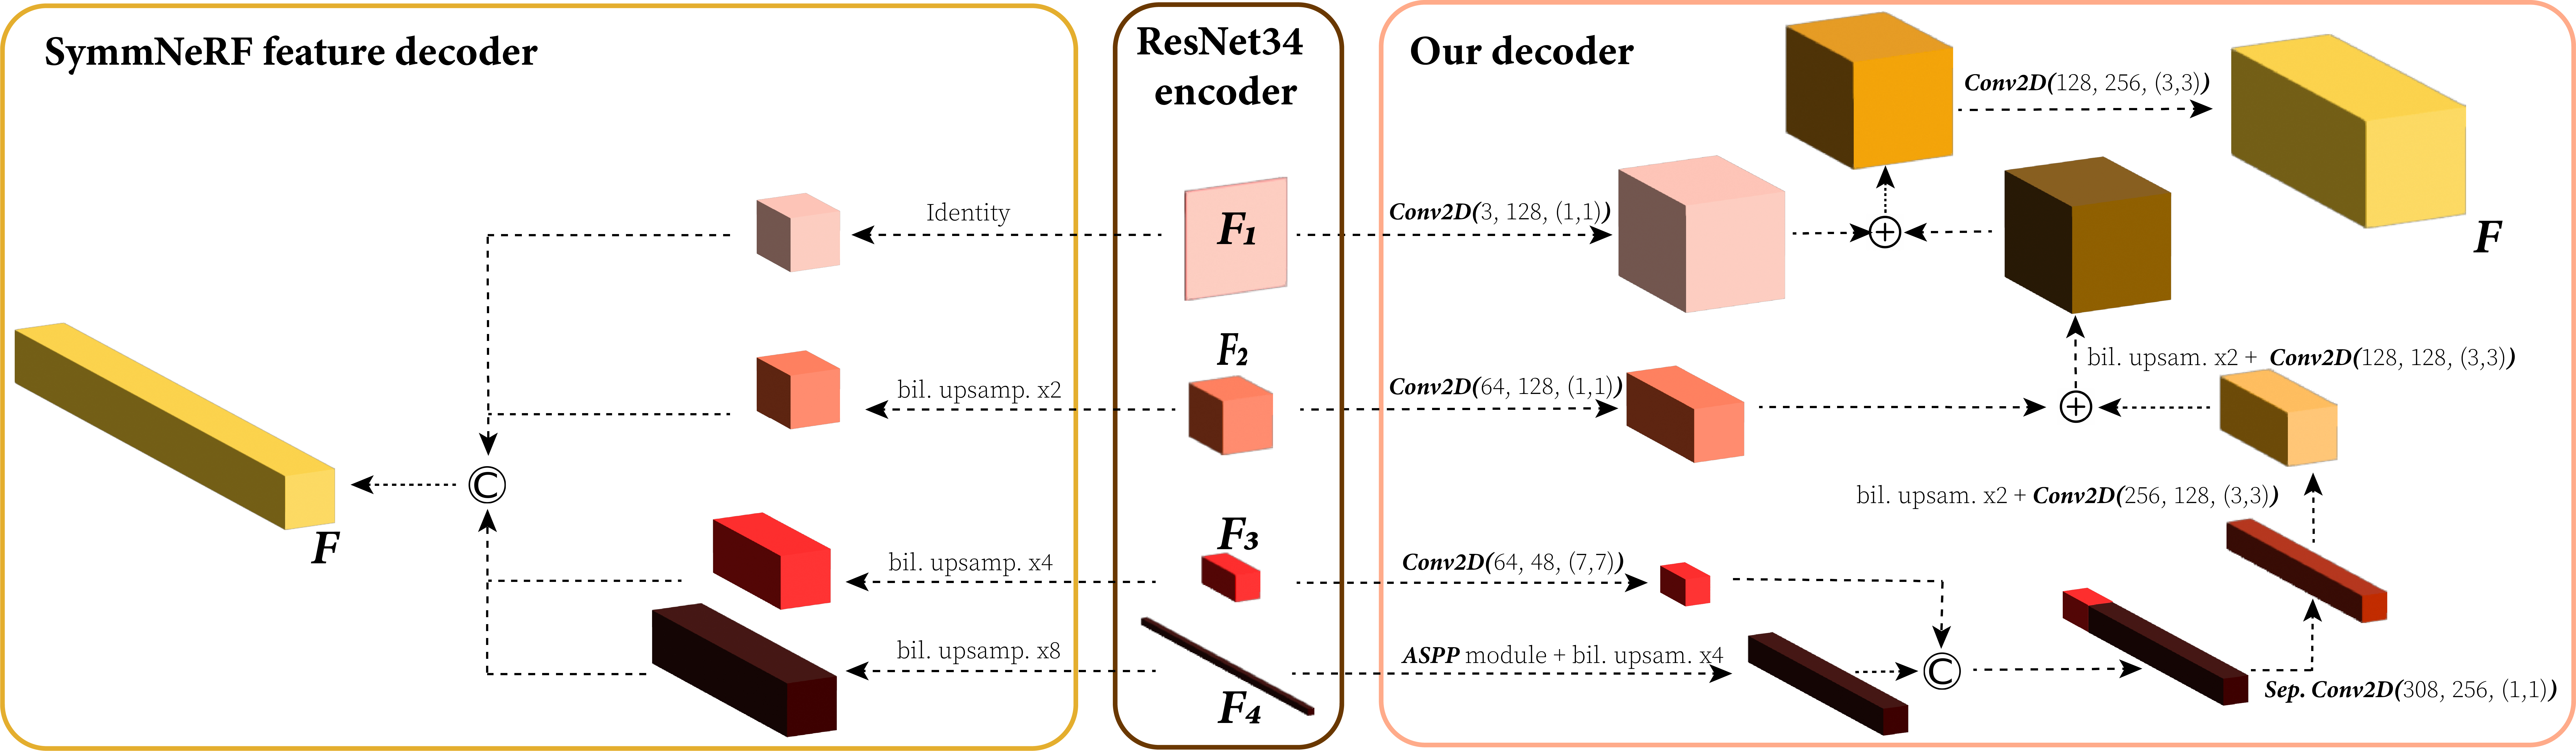
\includegraphics[width=\linewidth]{images/epinerf/feature_fusion_encoder.png}
  \end{center}
     \caption{Overview of the CNN decoder $\chi$ involved in SymmNeRF (left) and in our configuration by leveraging on DeepLabV3+ (right). One might note that $\chi$ in both case leverages a ResNet34-based encoder ~\cite{he2016deep}. }
  \label{fig:feature_encoder}
  \end{figure*}

We present on Figure \ref{fig:feature_illustration} few first-channel feature volumes, obtained from different \textit{Cars} and \textit{Chairs} instances.  High resolution feature volume allow to accurately perform pixel wise local sampling. Getting a low resolution feature volume such as the one involved in SymmNeRF result coarser pixel sampling. 

\begin{figure*}[h!]
\begin{center}
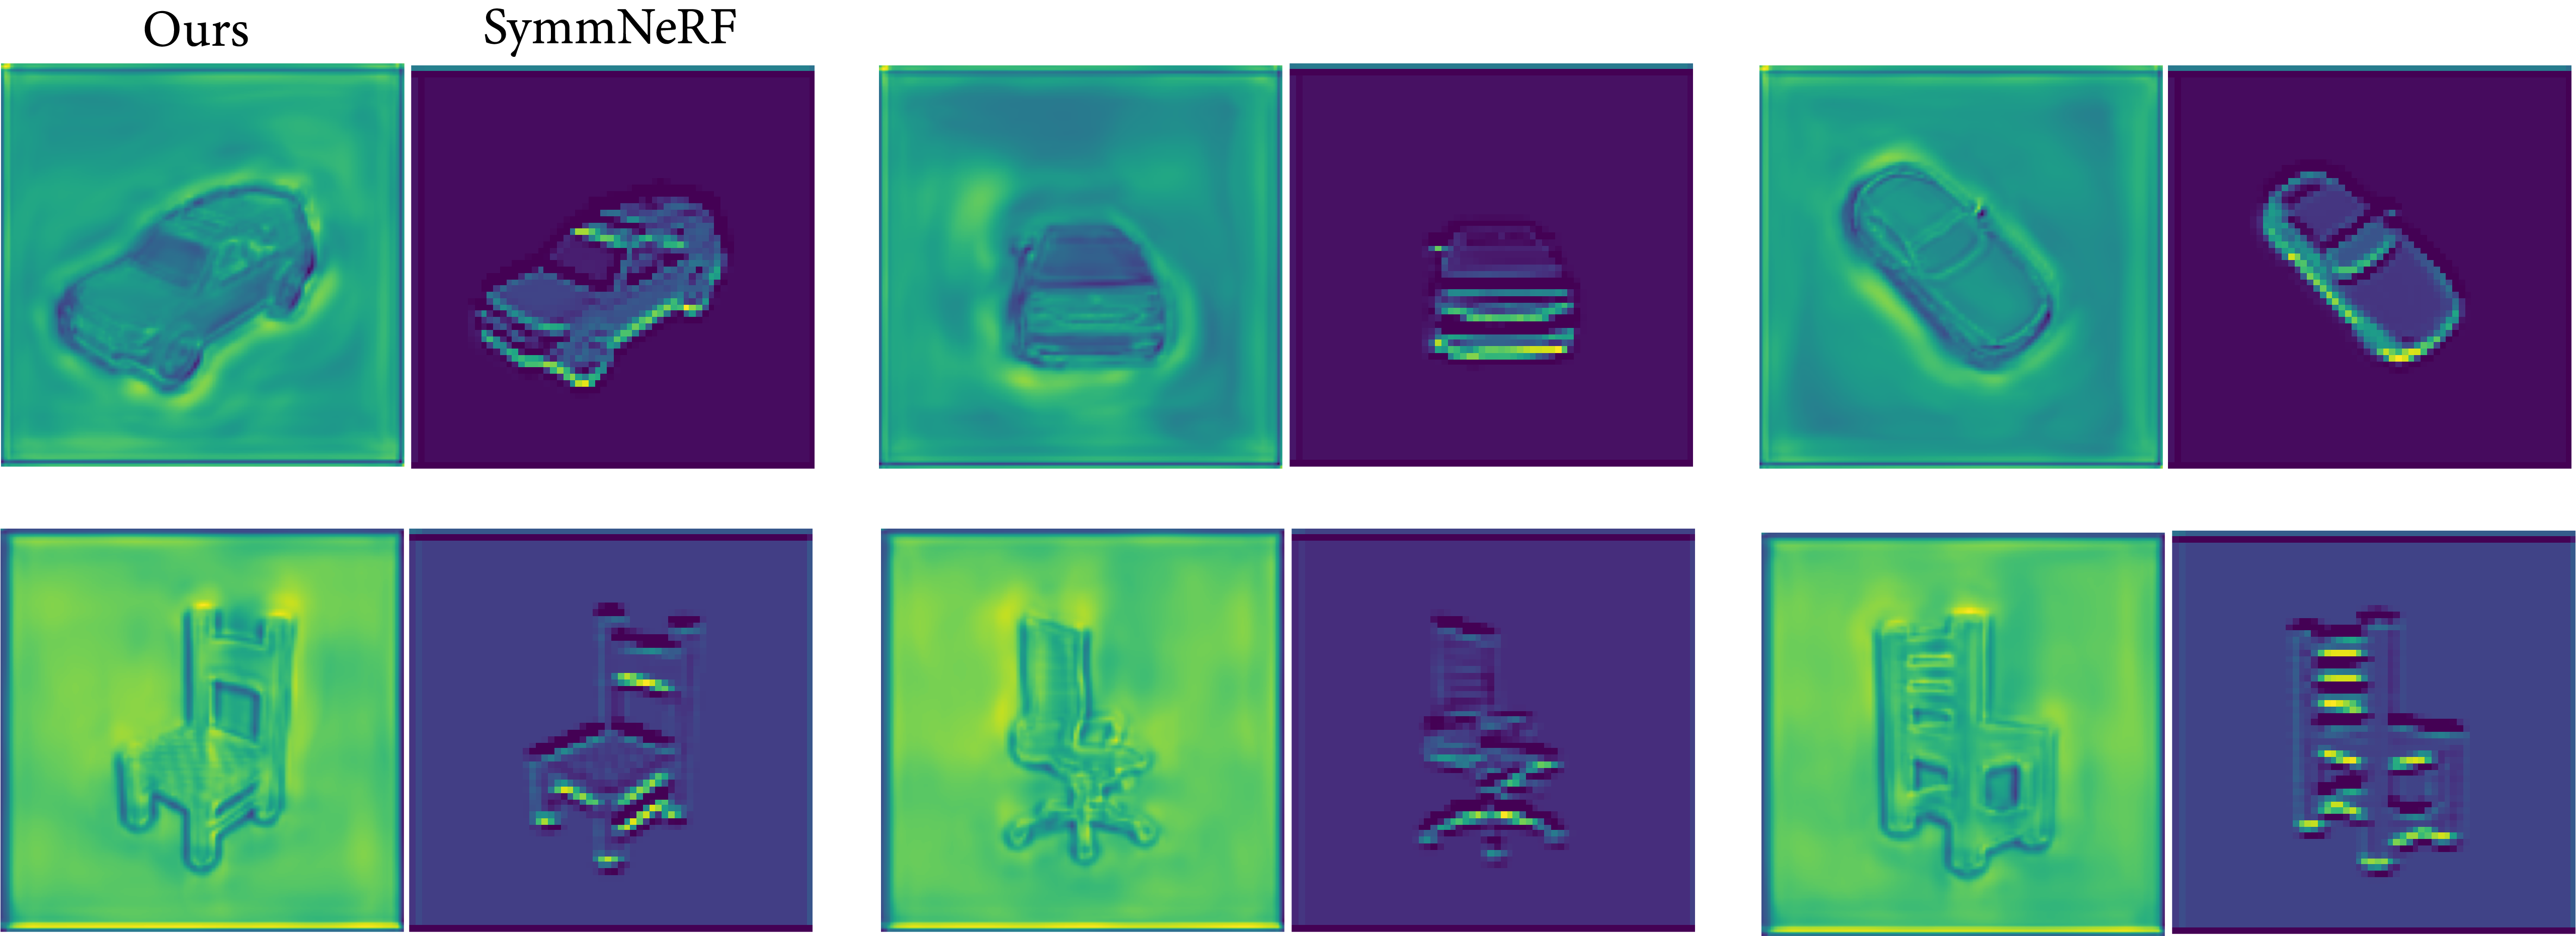
\includegraphics[width=.85\linewidth]{images/epinerf/feature_supp.png}
\end{center}
   \caption{Feature map produced by our encoder has a 128$\times$128 spatial resolution contrary to SymmNeRF one, which has a low  64$\times$64 resolution. Features produced by $\chi$ have tiny and complex patterns structure which SymmNeRF cannot deal with at half the input image size resolution.}
\label{fig:feature_illustration}
\end{figure*}

\noindent\textbf{Local and global NeRF conditioning.} Our CNN encoder-decoder $\chi$ primarily produces an intermediate set of features $(\mathbf{F}_{1},\mathbf{F}_{2},\mathbf{F}_{3},\mathbf{F}_{4})$ from $\textbf{I}_{s}$. While $\mathbf{F}_{s}$ must be considering as a \textit{local} input conditioning of the radiance fields (since feature are pixel-wise sampled during the perspective projection), we leveraged on an additional MLP network, called a hypernetwork $\Gamma$. Following prior works \cite{SRN,symmnerf}, such a hypernetwork $\Gamma$ is intended to learn the RGB radiance field weights $\theta_{NeRF_{\Phi}}$ during training. It takes as input a latent code $\mathbf{z}$, that is obtained from a non-linear projection of $\mathbf{F}_{4}$:

\begin{equation}
  \Gamma(\mathbf{z}) = \theta_{NeRF_{\Phi}} 
\end{equation}

The complete output of our CNN encoder-decoder $\chi$ can thus be re-written as:

\begin{equation}
    \textbf{z}, \textbf{F}_{s} = \chi(I_{s})
\end{equation}

An overview of hypernetwork $\Gamma$ and the way it interacts with $\Phi$ is depicted on Figure \ref{fig:supp_hyper_nerf}.

\begin{figure}[htp!]
  \begin{center}
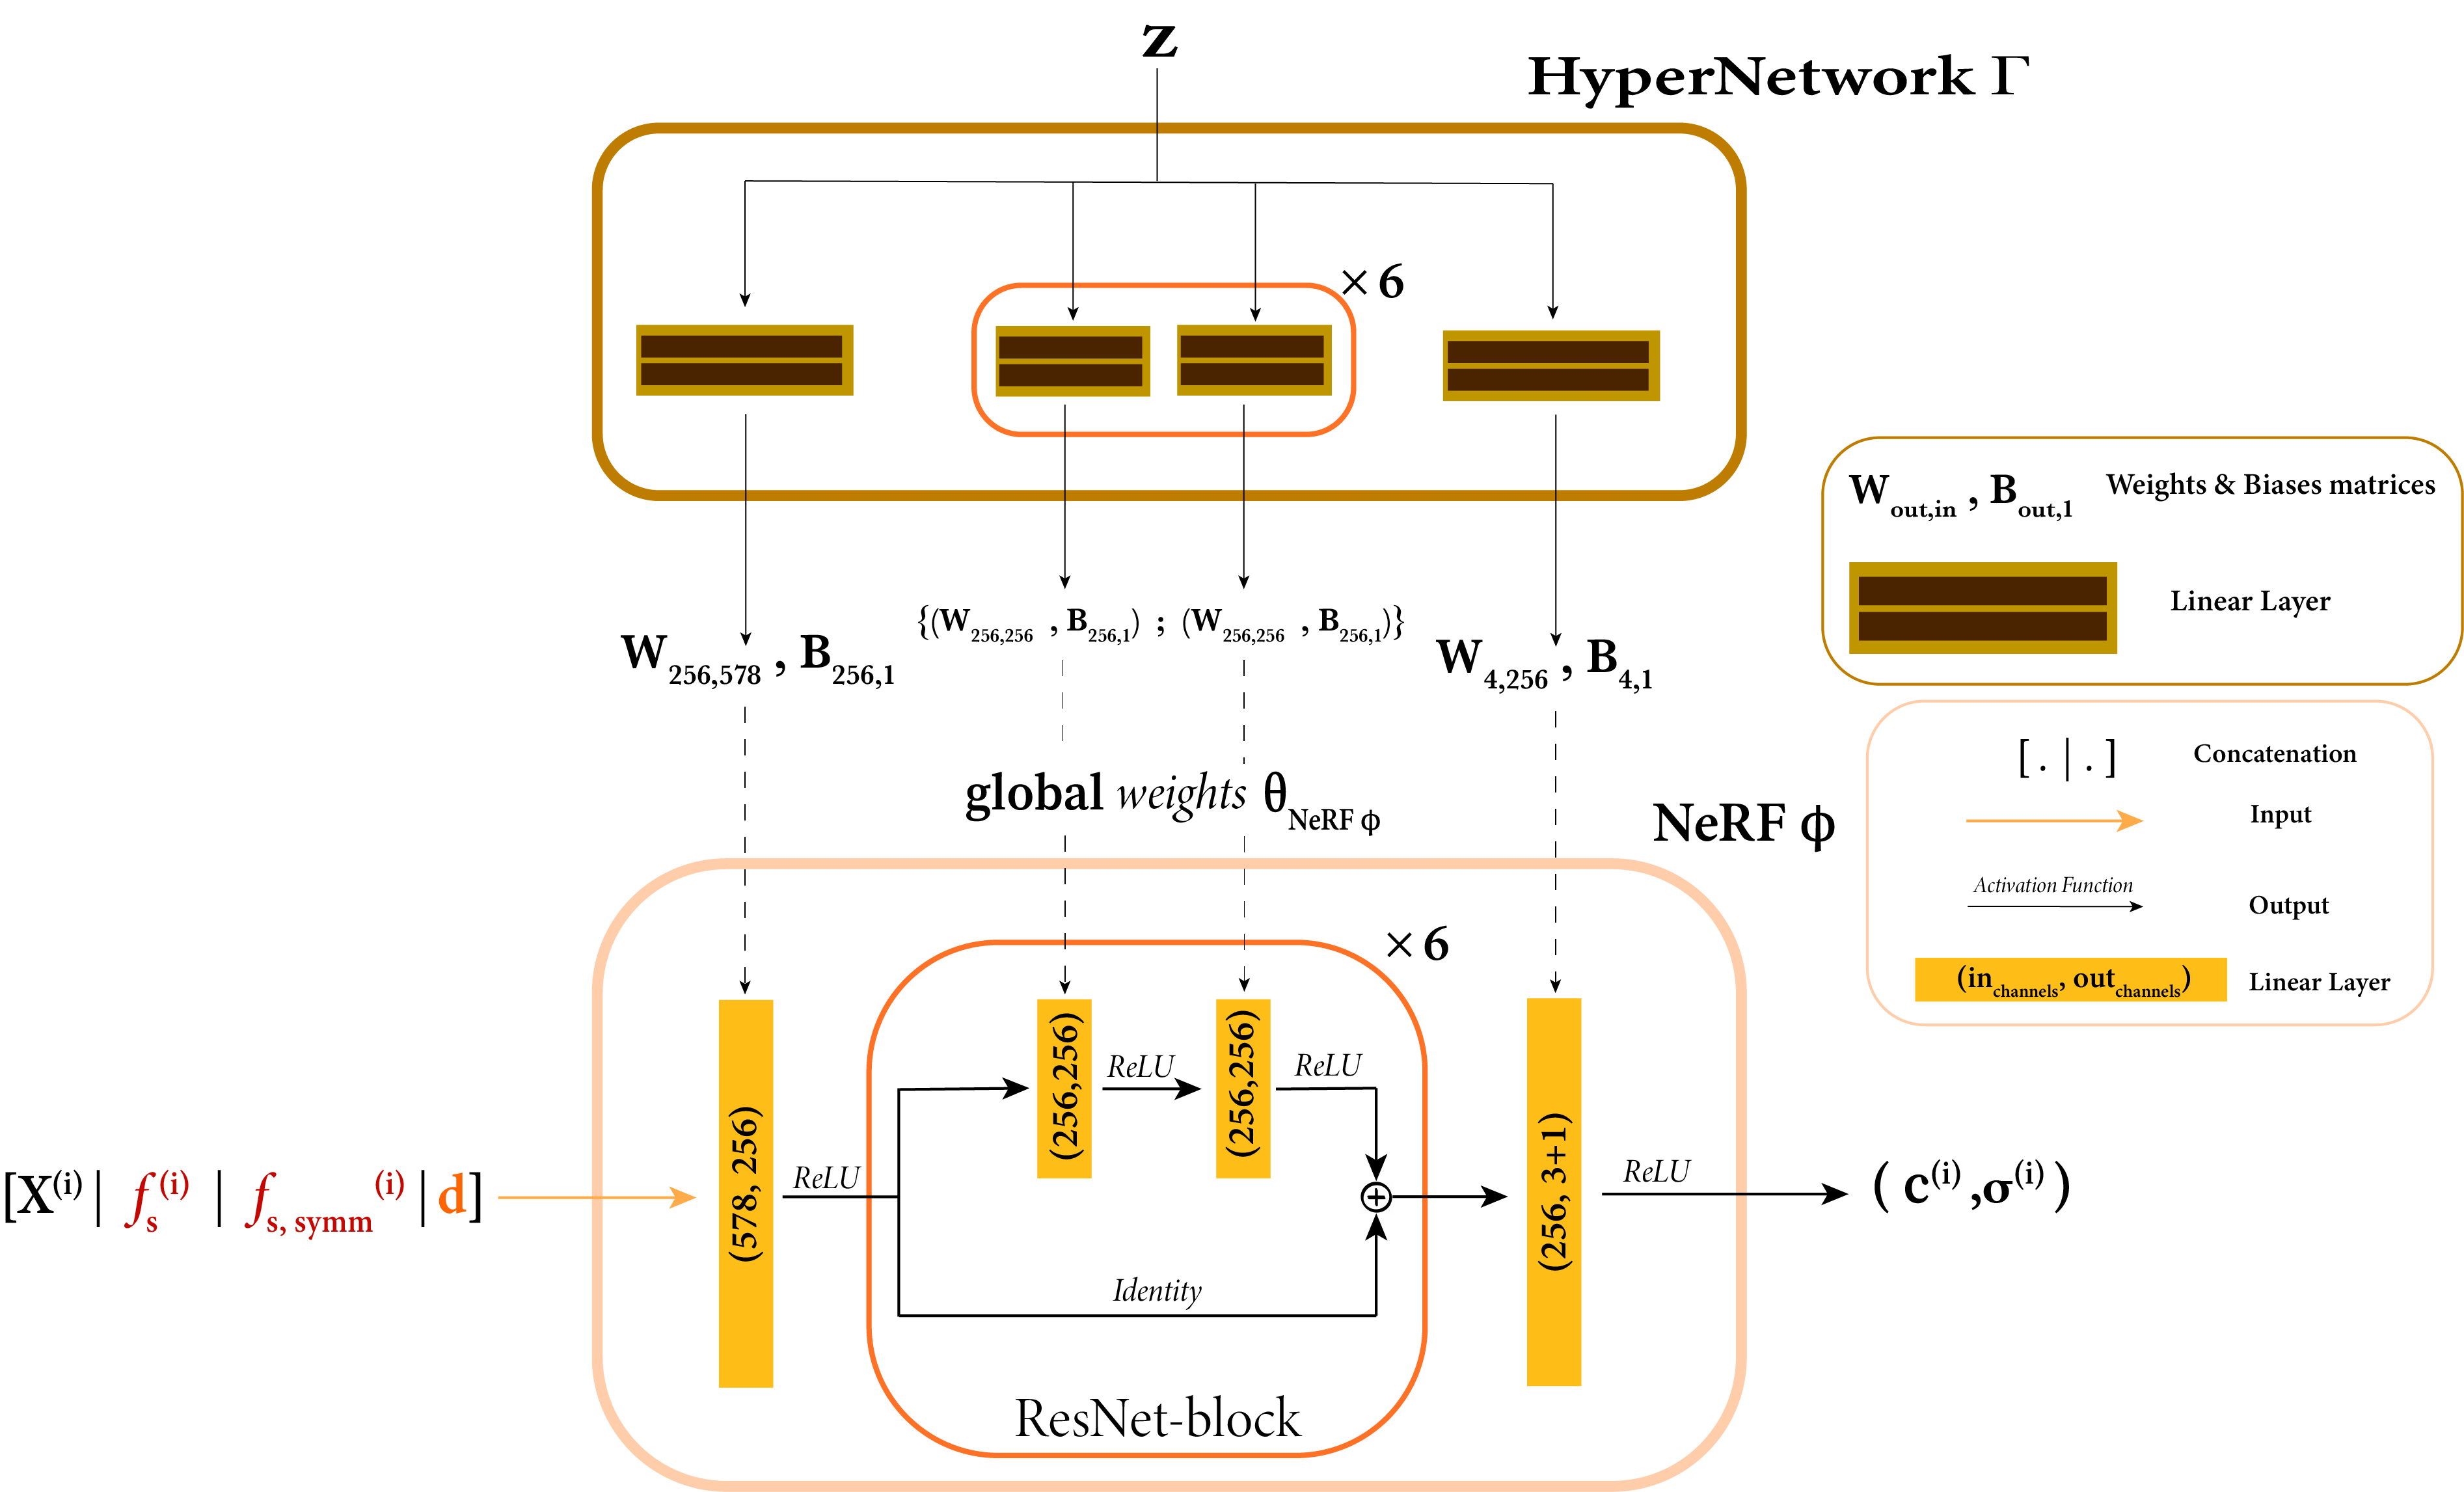
\includegraphics[width=\linewidth]{images/epinerf/supp_hyper_nerf.png}
\caption{HyperNetwork $\Gamma$ is trained to predict  the finite set of $\Phi$ weights. It indirectly acts as a global conditioning of the radiance field, in addition to the direct local conditioning offered by the source-aligned pixel-wise feature $f_{s}^{(i)},f_{s,symm}^{(i)}$.}
\label{fig:supp_hyper_nerf}
\end{center}
\end{figure} 

Since the radiance field is defined through its MLP-based architecture $\Phi$, $\theta_{NeRF_{\Phi}}$ represents a finite set of weight and bias matrices that $\Gamma$ can learn to predict given the deep latent code $\mathbf{z}$. Using such a Hypernetwork to predict the NeRF's weights $\theta_{NeRF_{\Phi}}$ is a way to globally condition $\Phi$, in addition to the local conditioning offered by the symmetric feature set $(f_{s},f_{s,symm})$.   

Primary role of $\Gamma$ is therefore to model NeRF weights distribution according to a single source image. Hypernetwork $\Gamma$ does not have to be trained with a specific loss objective: its weights are updated during back-propagation through the $\mathcal{L}_{2}$ loss function defined over the sampled RGB pixels (Alg. \ref{alg:fourth}). 

$\Phi$ is thus  both \textit{locally} (on its input) and  \textit{globally} (through its weights) conditioned: 
\begin{equation}
     \Phi_{\theta}(\mathbf{x}^{(i)},\mathbf{d},f_{s}^{(i)},f_{t}) = (\sigma^{(i)},\mathbf{c}^{(i)}) \hspace{.5cm}\text{;}\hspace{.5cm}  \theta = \Gamma(\mathbf{z})
\end{equation}


\noindent\textbf{Symmetry prior integration.}
Following SymmNeRF ~\citep{li2022symmnerf} prior work, we made the assumption the (YZ) plane in the canonical coordinates system was a symmetry plane for the implicit 3D scenes we are aiming to reconstruct. A 3D point $\mathbf{x}$ along a target ray \textbf{r} thus has a symmetrical point with respect to the (YZ)-symmetry plane through:
\begin{equation}
    \mathbf{x}^{(i)}_{symm} = \mathbf{M}\mathbf{x}^{(i)}
\end{equation}
where $\mathbf{M} = \mathbf{I}_{4}\footnote{the Identity matrix in $\mathbb{R}^{4}$} - 2e_{1}e_{1}^{T}$ and $e_{1}$ the first 3D unit basis vector. Such a symmetrical 3D point is back-projected on the source-aligned feature volume $\mathbf{F}_{s}$. The \textit{local} deep feature fed to the NeRF $\Phi$ is finally: 
\begin{equation}
    f^{(i)} = concat\left(f_{s}^{(i)}, f_{s,symm}^{(i)}\right)
\end{equation}

\noindent\textbf{Training.} As depicted on Figure \ref{fig:overview}, our EpiNeRF architecture has a three-step training procedure. It integrates a feature radiance field, termed NeRFeature $\Psi$, in combination with a CNN-based encoder-decoder $\chi$ that \textit{locally} condition the main RGB radiance fields $\Phi$ through an epipolar based attention mechanism. A hypernetwork $\Gamma$ also \textit{globally} conditions $\Phi$, by predicting its learnable parameters through a lightweight MLP network. 

Considering a training set of N objects $\{\mathcal{D}\}_{i=1}^{N}$ with V different viewpoints $\mathcal{D}^{(i)} = \{I_{i}^{(j)},\pi_{i}^{(j)}\}_{j=1}^{V}$ per instance and a batch of rays $\mathcal{R}$, EpiNeRF is optimised through the loss functions: 
\begin{equation}
 \min_{\Psi} \sum_{i}\sum_{j}\mathcal{L}_{\Psi}\left(I_{i}^{(j)},\pi_{i}^{(j)},\Psi,\chi \right) \hspace{.2cm} ; \hspace{.2cm}\mathcal{L}_{\Psi}= \sum_{\mathbf{r}\in\mathcal{R}} || f_{t}(\mathbf{r}) - f_{t}^{(GT)}(\mathbf{r}) ||_{2}^{2}
\end{equation}
and 
\begin{equation}
 \min_{\zeta=\{\chi,\Phi,\Gamma\}}\sum_{i}\sum_{j}\mathcal{L}_{\zeta}\left(I_{i}^{(j)},\pi_{i}^{(j)},\Psi,\zeta \right)\hspace{.2cm}  ; \hspace{.2cm}\mathcal{L}_{\zeta}= \sum_{\mathbf{r}\in\mathcal{R}} || c(\mathbf{r}) - c^{(GT)}(\mathbf{r}) ||_{2}^{2}
\end{equation}


where $c^{(GT)}(\mathbf{r})$ represents the ground truth pixel that was sampled on $\mathbf{I}_{t}$, $f^{(GT)}(\mathbf{r})$ the \textit{pseudo} ground truth deep feature that was sampled $F_{t}=\chi(I_{t})$.


Deep features produced by NeRFeature are implicitly conditioned by $\chi$ since the source aligned feature $f_s^{(i)}$ is fed as input. 

\section{Experiments}
\subsection{View synthesis on synthetic data - SRN ShapeNet}
Presented results were obtained on the ShapeNet dataset ~\citep{chang2015shapenet}, by focusing on the ShapeNet-SRN ~\citep{sitzmann2019scene} version. The \textit{Cars} and \textit{Chairs} classes respectively have 3514 and 6591 objects. Training is performed over the 50 different views per instance, while the testing set has 251 views per object, sampled on an Archimedean spiral.\newline

Our method reaches state-of-the-art performances according to Table \ref{table:comp_res} and even outperforms the heavier transformer-based architecture ~\citep{lin2023vision} on almost all metrics. 

\begin{table}[h!]
\caption{Comparisons against state of the art methods on the category specific \textit{Chairs} and \textit{Cars} classes from the ShapeNet-SRN dataset. Best results are highlighted in red, second ones in orange and third ones in yellow. }
\label{table:comp_res}
\begin{center}%\centering%
\begin{adjustbox}{width = \linewidth}
\begin{tabular}[h]{c||ccccccc}
\hline
 Method & \multicolumn{3}{c}{Car} & \multicolumn{3}{c}{Chair} \\
 &  SSIM ($\uparrow$) & PSNR ($\uparrow$) & LPIPS ($\downarrow$) & SSIM ($\uparrow$) & PSNR ($\uparrow$)) & LPIPS ($\downarrow$)\\
\hline
SRN ~\citep{sitzmann2019scene}& \cellcolor{yellow!25}0.89 & 22.25 & 0.129 & 0.89 & 22.89 & 0.104\\
PixelNeRF ~\citep{yu2021pixelnerf} & \cellcolor{orange!25}0.90 & 23.17 & 0.146 & \cellcolor{yellow!25}0.91 & 23.72 & 0.128\\
FE-NVS ~\citep{guo2022fast} & \cellcolor{red!25}0.91 & 22.83 & \cellcolor{yellow!25}0.099 & \cellcolor{orange!25}0.92 & 23.21 & 0.077 \\
GeNVS~\citep{chan2023genvs}& \cellcolor{yellow!25}0.89 & 20.7 & 0.104 & - & - & - \\
ShaRF ~\citep{rematas2021sharf} & \cellcolor{orange!25}0.90 & 22.90 & - & \cellcolor{orange!25}0.92 & 23.37 & - \\
CodeNeRF ~\citep{jang2021codenerf} & \cellcolor{red!25}0.91 & \cellcolor{orange!25}23.80 & - & 0.90 & 23.66 & -  \\
SymmNeRF\footnotemark~\citep{li2022symmnerf}& \cellcolor{orange!25}0.90 & \cellcolor{yellow!25}23.10 & 0.110 & \cellcolor{yellow!25}0.91 & \cellcolor{yellow!25}24.14  & \cellcolor{orange!25}0.075 \\
VisionNeRF ~\citep{lin2023vision} & \cellcolor{red!25}0.91 & 22.88 & \cellcolor{red!25}0.084 & \cellcolor{red!25}0.93 & \cellcolor{orange!25}24.48  & \cellcolor{yellow!25}0.077 \\
Ours &\cellcolor{red!25} 0.91 & \cellcolor{red!25} 24.01  &\cellcolor{orange!25}  0.086 &  \cellcolor{orange!25}0.92   & \cellcolor{red!25}24.60&  \cellcolor{red!25}0.070 \\

\hline 
\end{tabular}
\end{adjustbox}
\end{center}
\end{table}
\footnotetext[3]{SymmNeRF~\citep{li2022symmnerf} results differ from the ones originally reported by authors since we had to retrain their architecture.}

As depicted in Figures \ref{fig:exp-srn-cars} and \ref{fig:exp-srn-chairs}, EpiNeRF successfully gathers best aspects of both SymmNeRF ~\citep{li2022symmnerf} and VisionNeRF~\citep{lin2023vision}. It renders novel views that are simultaneously sharp (eased by the ViT in VisionNeRF) and consistent from a symmetrical perspective on colour patterns (eased by the symmetry prior from SymmNeRF). In this regard, the gray stripe pattern on Figure \ref{fig:exp-srn-cars} (\textit{middle})is  accurately synthesized by our architecture, contrary to concurrent works that either fail to synthesise sharp views (SymmNeRF) or grasp the inherent symmetrical band (VisionNeRF). 

\begin{figure}[h!]
    \begin{center}
  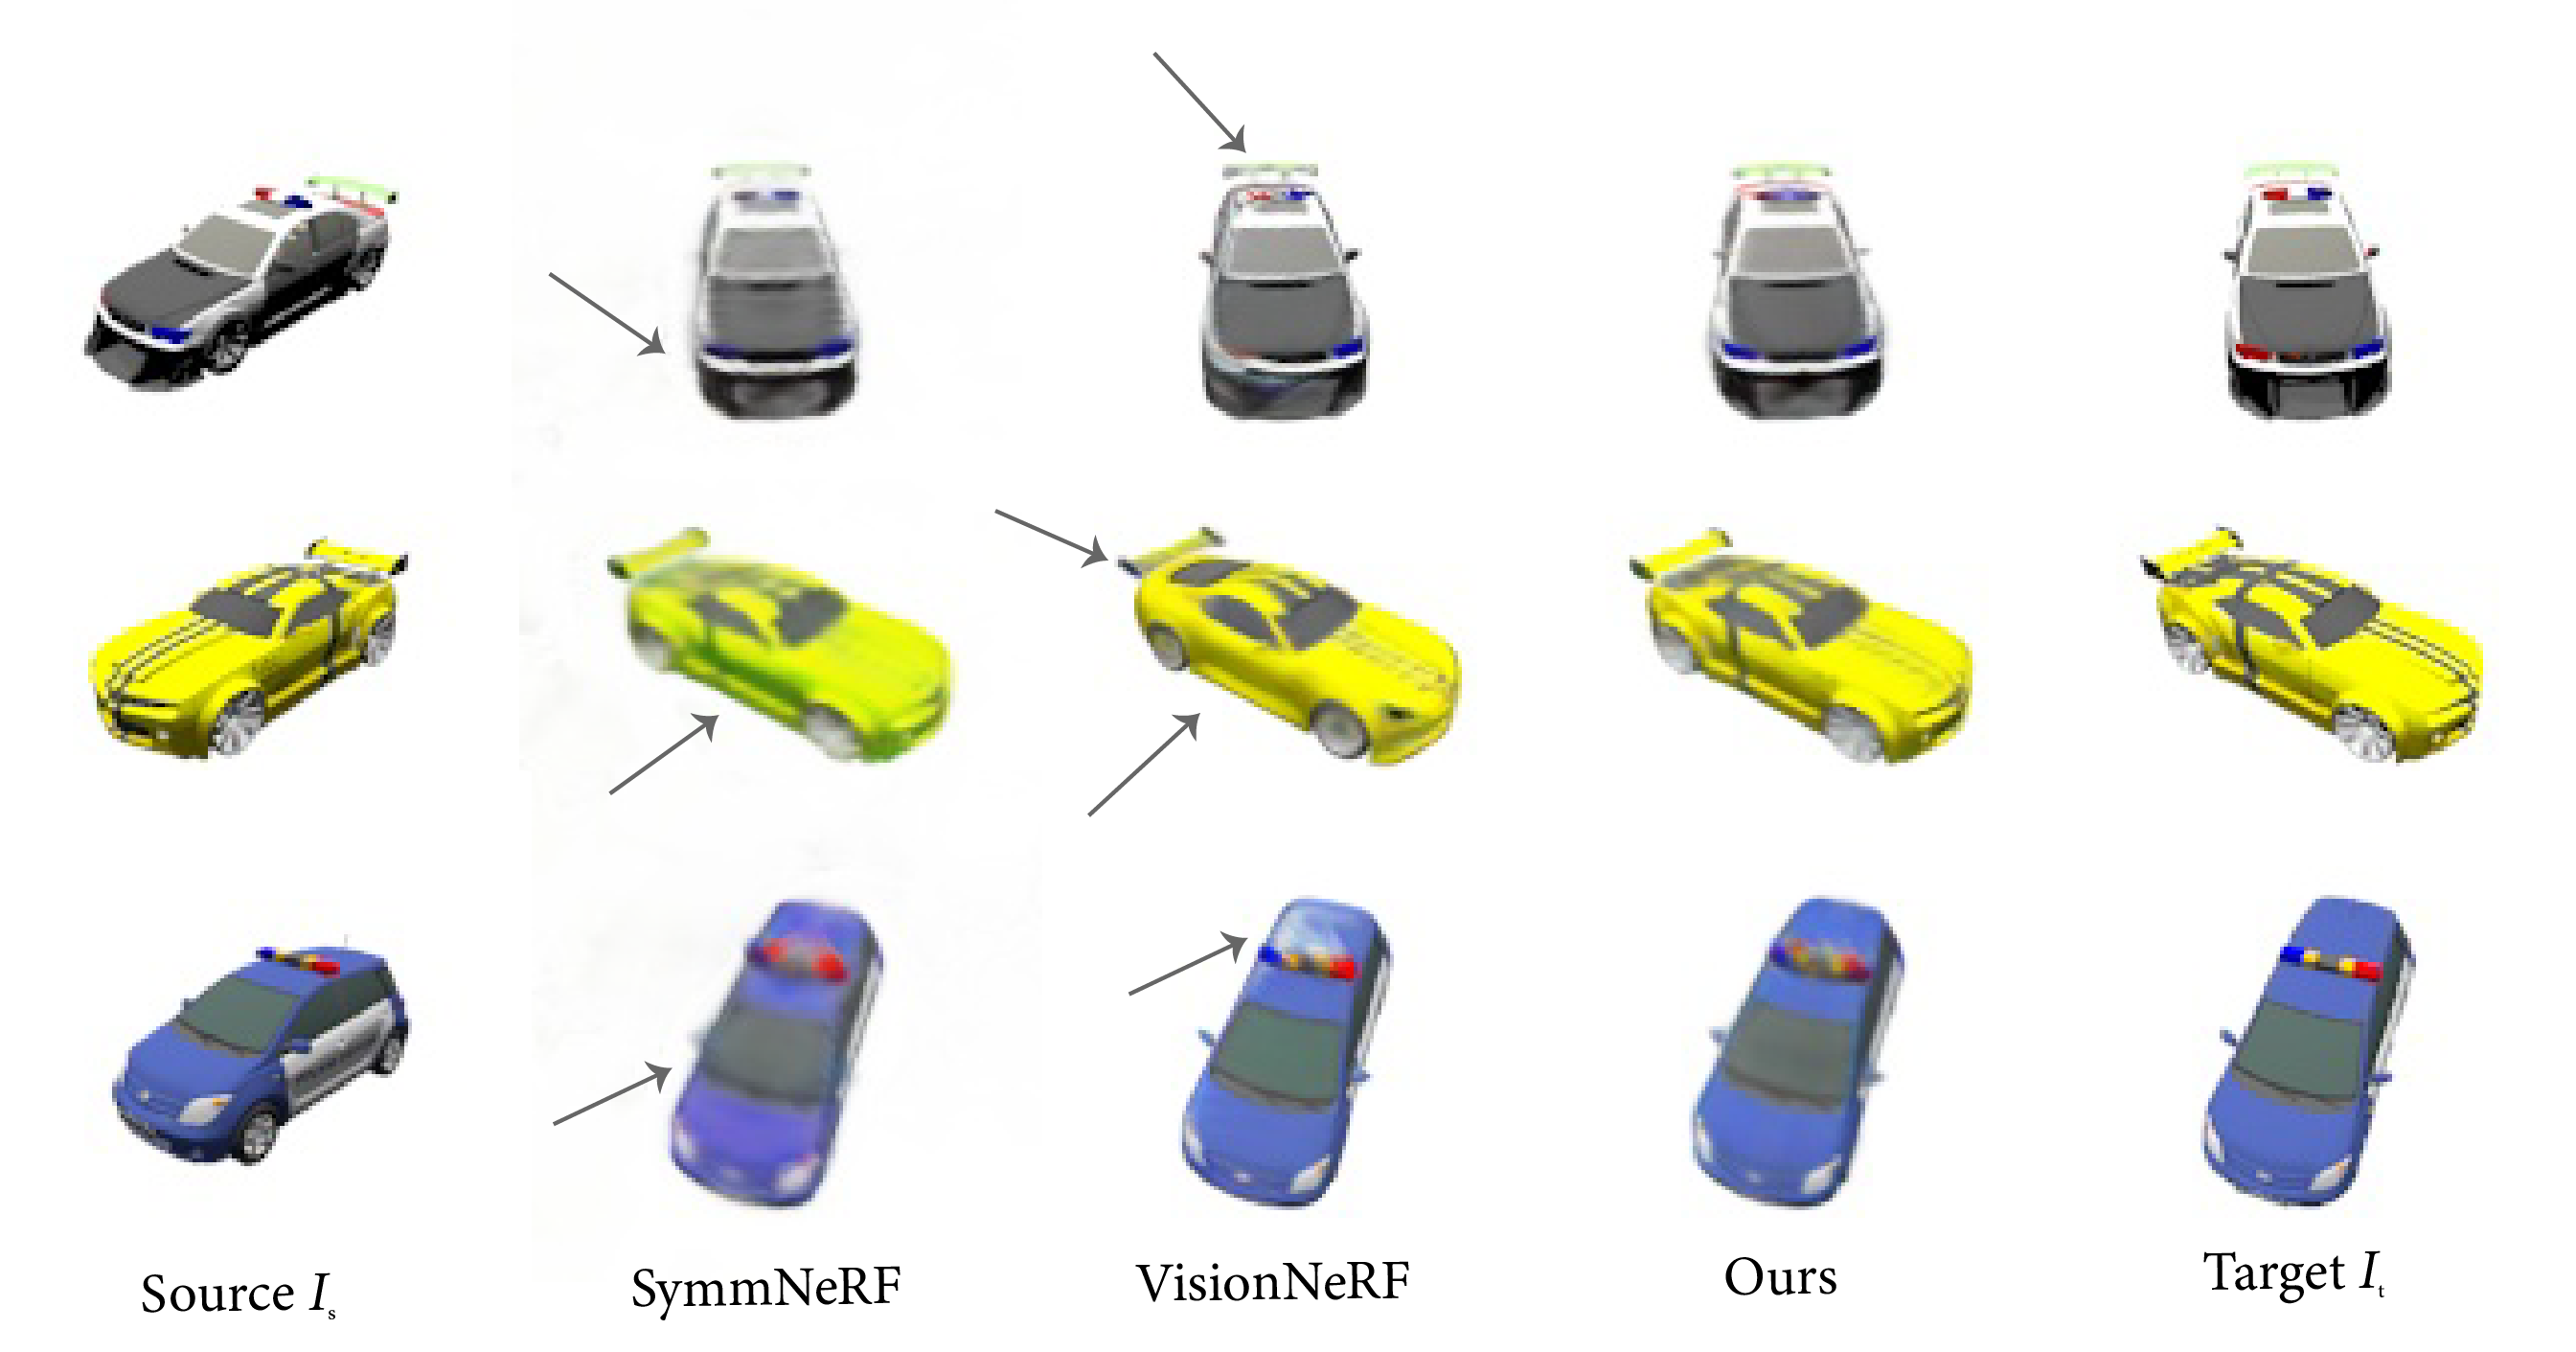
\includegraphics[width=\linewidth]{images/epinerf/cars_BMVC.png}
  \end{center}
  \caption{\textbf{Novel view synthesis on the ShapeNet category-specific} \textit{Cars}. Our method allows to render sharper novel views than SymmNeRF ~\citep{li2022symmnerf} while maintaining the symmetry that VisionNeRF ~\citep{lin2023vision} fails to preserve.}
  \label{fig:exp-srn-cars}
\end{figure}

\begin{figure}[h!]
    \begin{center}
  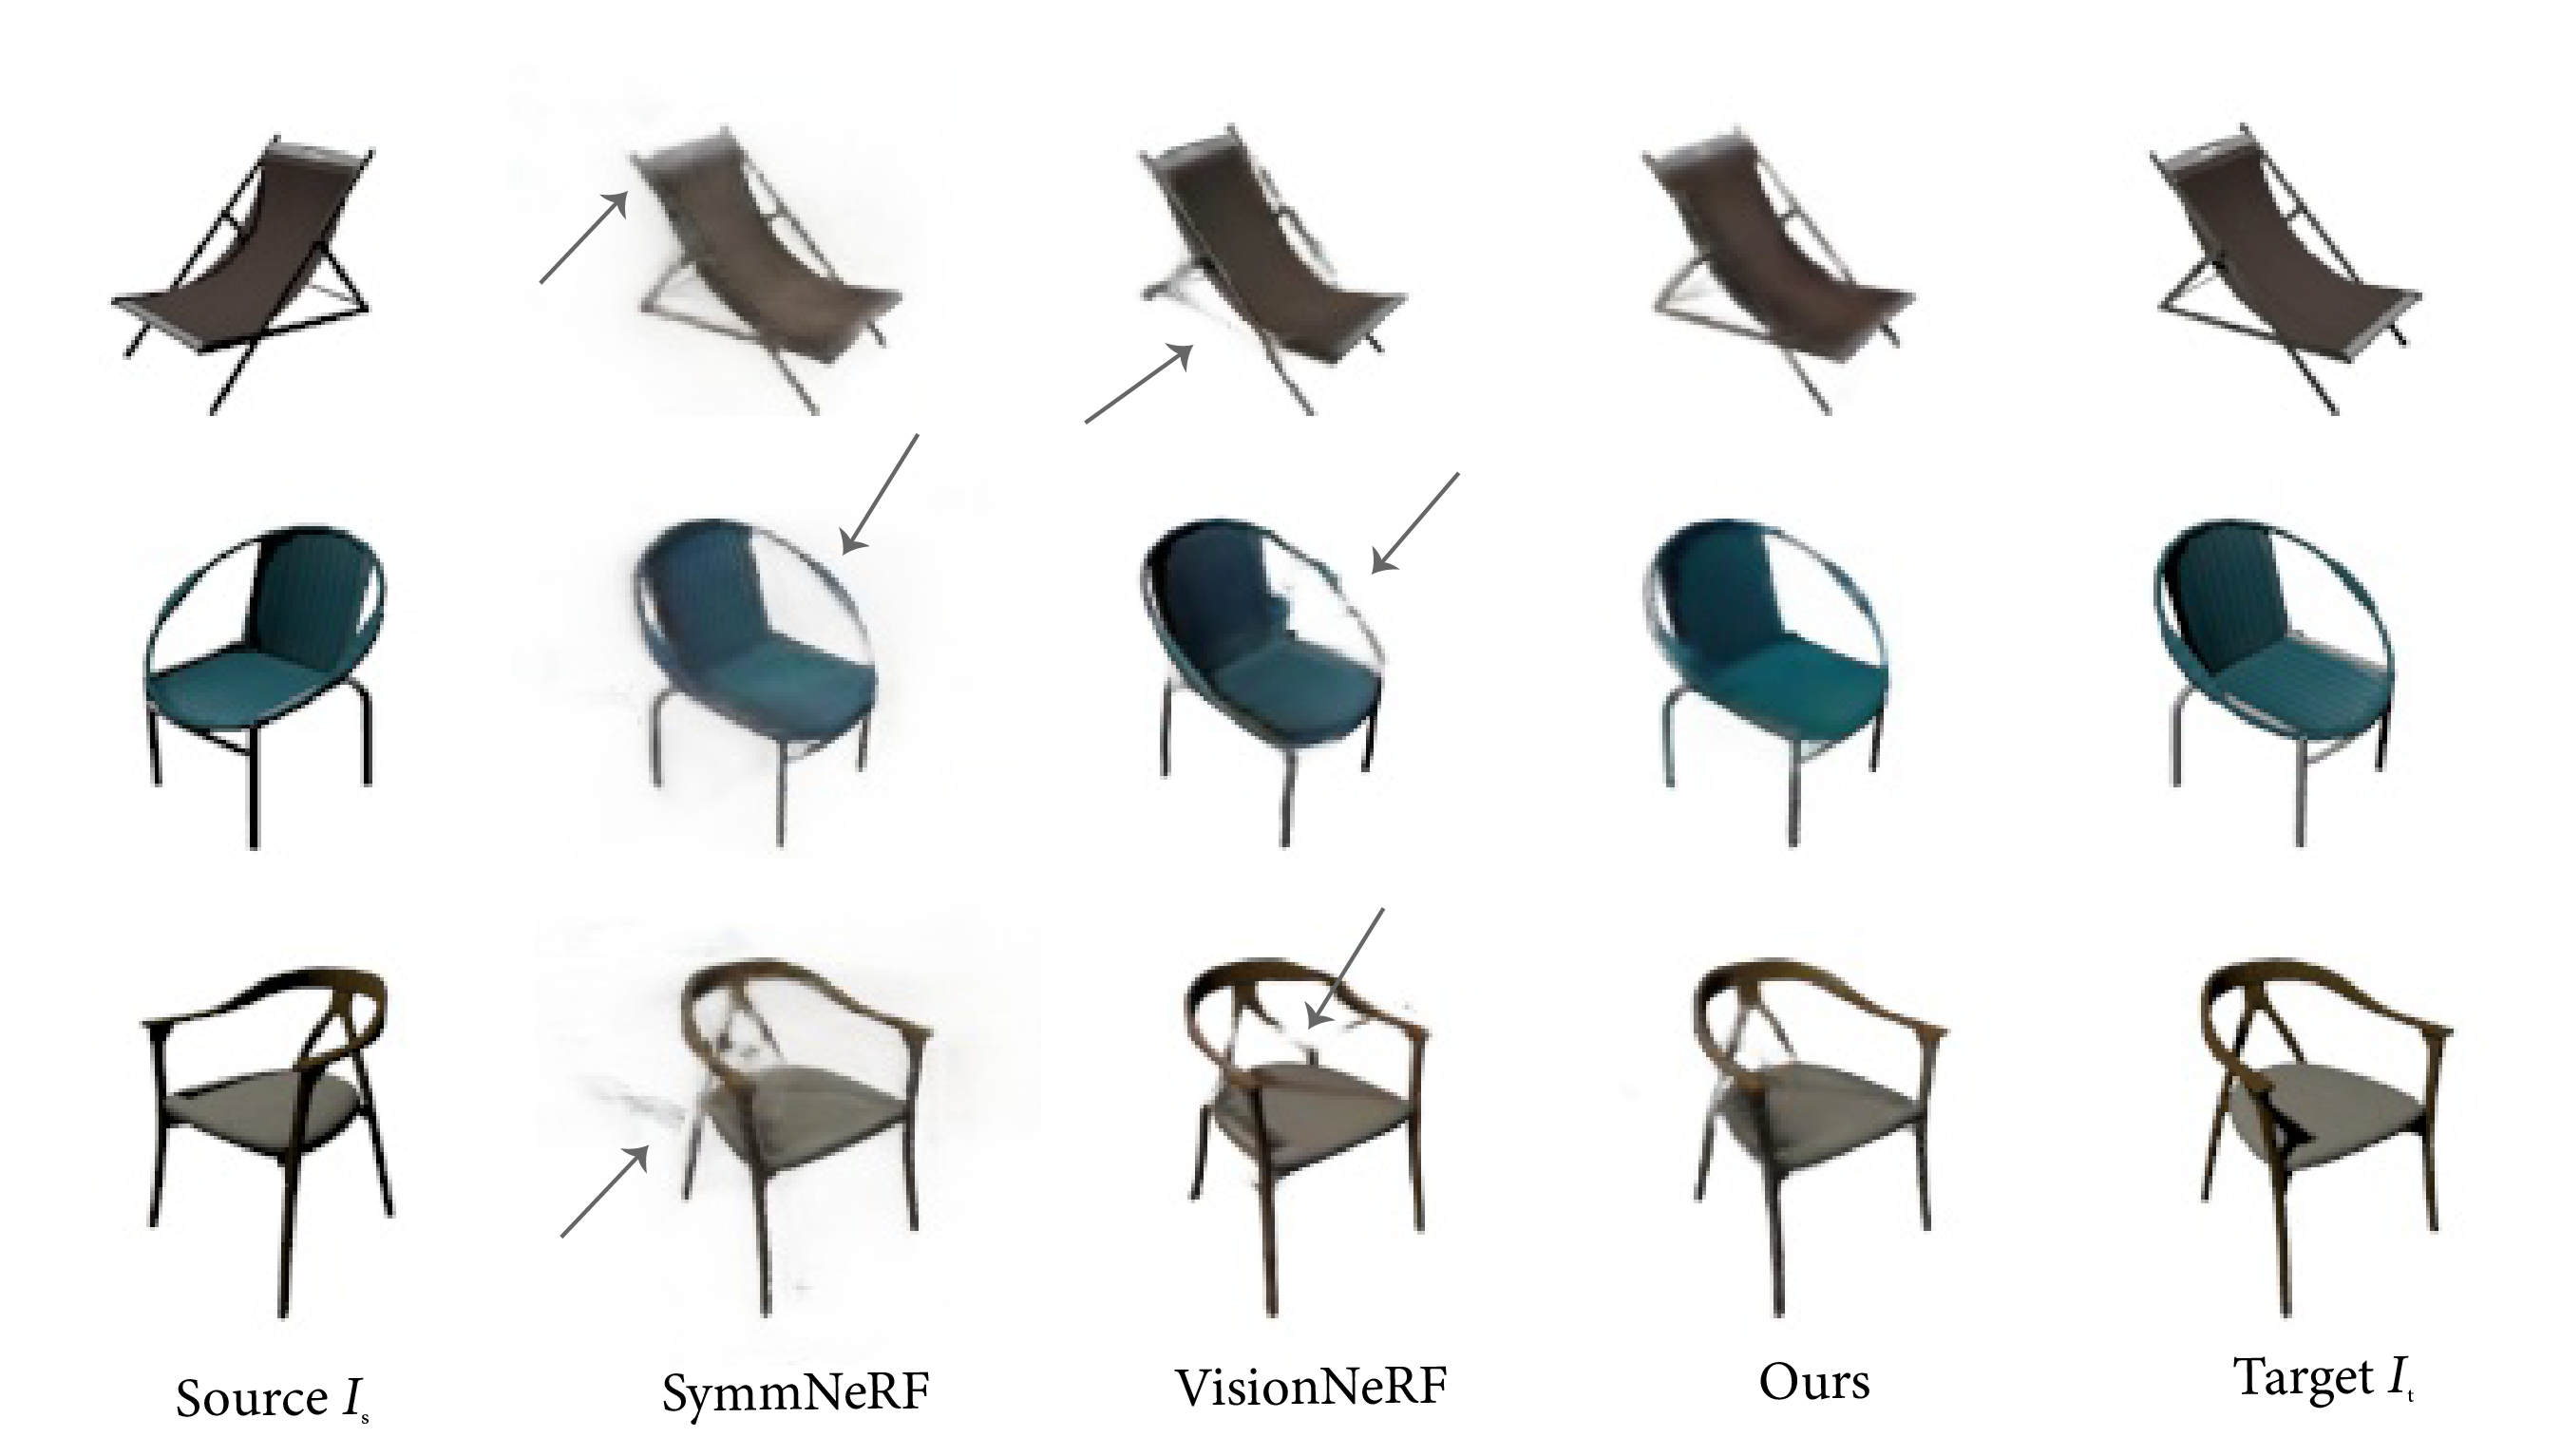
\includegraphics[width=\linewidth]{images/epinerf/chairs_BMVC.png}
  \end{center}
  \caption{\textbf{Novel view synthesis on the ShapeNet category-specific} \textit{Chairs}. Complex armrest structures are barely rendered by SymmNeRF \citep{li2022symmnerf} and VisionNeRF \citep{lin2023vision}, contrary to EpiNeRF. }
  \label{fig:exp-srn-chairs}
\end{figure}
 Similar observations can be drawn from the \textit{Chairs} class in Figure \ref{fig:exp-srn-chairs}. Intricate geometry on the back and armrests is not entirely synthesised by VisionNeRF  which fails to apprehend how symmetric a chair can be: the armrest structure on the first row is partially missing in the rendered view, even though all the visual information was provided in the source view to render it. 

 Results on real-world dataset such as Stanford Cars dataset \citep{krause20133d} are readely available in the supplementary material. 

\subsection{Ablation study}
Starting with a \textit{baseline} architecture that integrates no symmetry prior information, a vanilla bilinear upsampling strategy to produce $\mathbf{F}_{s}$ and no epipolar attention, we conducted an ablation study to show how each EpiNeRF's components behave on our final novel view rendering architecture. 

\begin{table}[htp!]
\caption{Influence of the different modules on EpiNeRF architecture.}
\label{tab:ablation}
\begin{center}
\centering
\begin{adjustbox}{width=\textwidth}
\begin{tabular}[h]{c||ccccccc}
\hline
Method & \multicolumn{3}{c}{Car} & \multicolumn{3}{c}{Chair} \\
 &  SSIM ($\uparrow$) & PSNR ($\uparrow$) & LPIPS ($\downarrow$) & SSIM ($\uparrow$) & PSNR ($\uparrow$)) & LPIPS ($\downarrow$)\\[.5pt]
\hline
baseline & 0.89 & 22.61 & 0.125 & 0.88 & 22.73 & 0.112  \\[1.5pt]
\hline 
+ Symmetry constraint ~\citep{li2022symmnerf}  & 0.89 & 23.07  & 0.122 & 0.89 & 23.66 & 0.102 \\
+ DeepLabV3 CNN encoder  & 0.91 & 23.84 & 0.101 & 0.89 & 23.60  & 0.124  \\
+ Epipolar Attention  & \cellcolor{red!25}0.91 & \cellcolor{red!25}24.01 &\cellcolor{red!25}0.086 & \cellcolor{red!25}0.92 &  \cellcolor{red!25}24.60 &\cellcolor{red!25}0.070 \\
\end{tabular}
\end{adjustbox}
\end{center}

\end{table}

As shown on Table \ref{tab:ablation} and visually confirmed in the supplementary material, each of our component consistently improve the \textit{baseline} architecture. Both the feature volume encoding with DeepLabV3 and the lightweight feature-based epipolar attention mechanism have a positive and significant influence over the rendered novel views. The symmetrical constraint helps to handle complex symetrical most ShapeNet objects have.  

We visually illustrate and complete on Figure \ref{fig:ablation} through two distinct novel views synthesis the ablation result table that was presented in the main paper. \newline 

\begin{figure}[h!]
    \begin{center}
  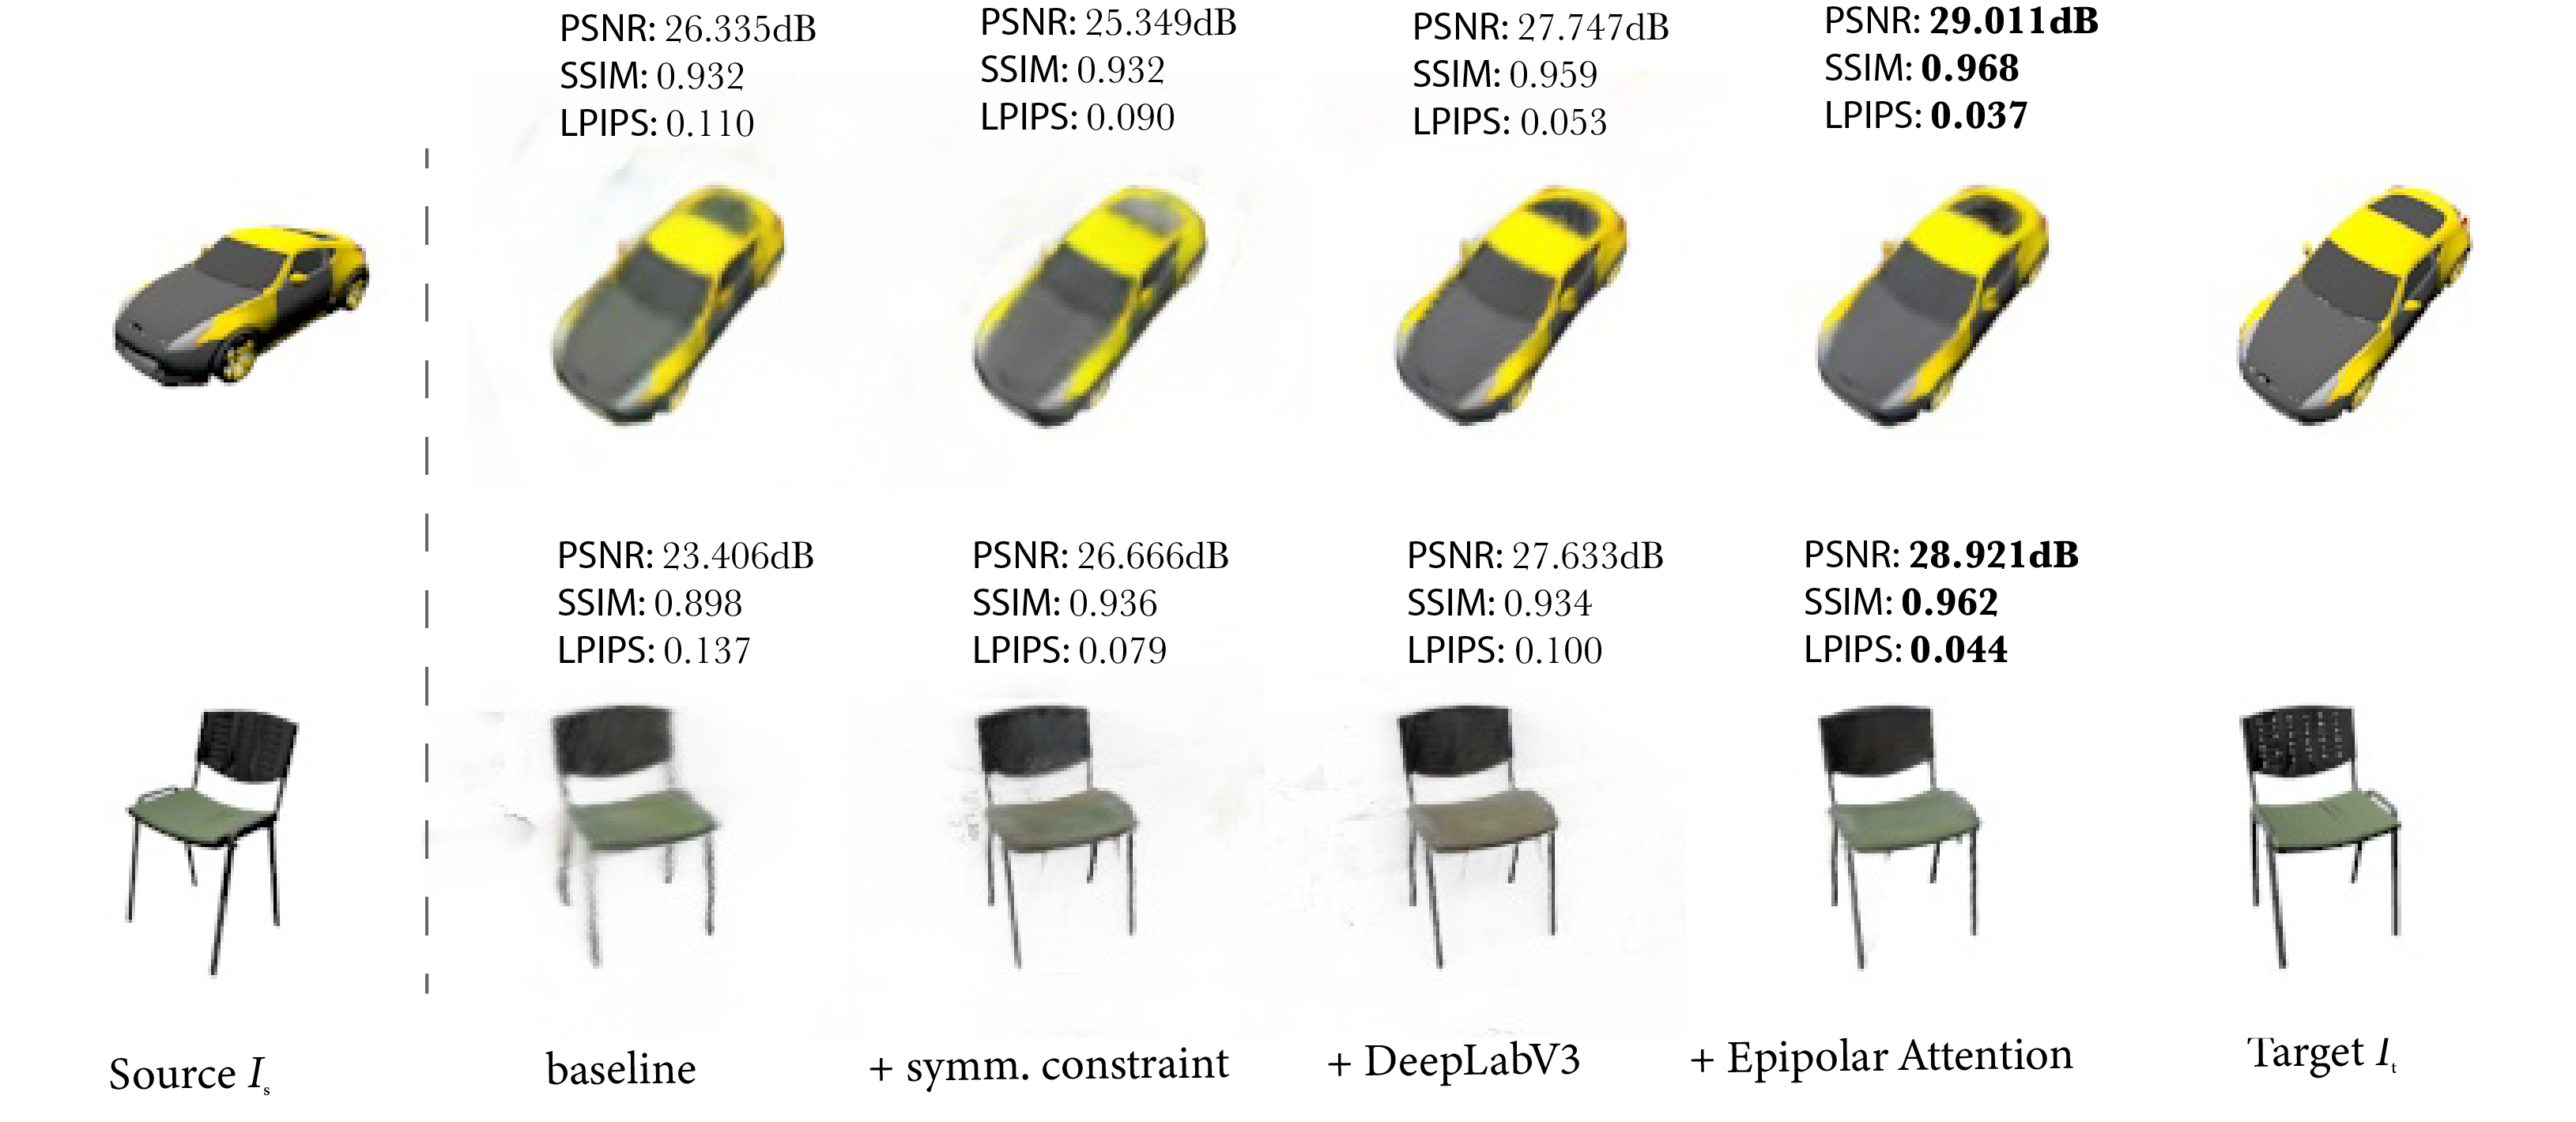
\includegraphics[width=\linewidth]{images/epinerf/supp_ablation_illustration.png}
  \caption{Visual influence of the different modules and constraints that were progressively applied to our architecture on ShapeNet-SRN dataset.}
  \label{fig:ablation}
  \end{center}
\end{figure}  

Integrating the symmetry prior helps the network to better grasp symmetrical and complex pattern structures, whereas the high-resolution feature volume produced by our encoder-decoder $\chi$ leads to sharper edges and thinner structures in RGB space. Finally, the feature attention-based epipolar module, that involved both source-aligned (from $\chi$) and target-aligned (from NeRFeature $\Psi$) features improves the overall quality of the EpiNeRF rendering.

\subsection{Feature and attention: visual insights}
\label{subsec:visual_insights}

\noindent \textbf{Target-aligned feature synthesis with NeRFeature.} 
Whereas primary purpose of NeRFeature is not to generate an entire feature map from a target viewpoint, a complete deep feature volume $\mathbf{F}_{t}$ is depicted on Figure \ref{fig:feat_and_att} (a) for an illustrative purpose. The overall target car pose is properly inferred by our feature radiance field $\Psi$, even through tiny details fails to be accurately retrieved (e.g windows). \newline

\begin{figure}[htp!]
\begin{center}
\begin{tabular}{cc}
\bmvaHangBox{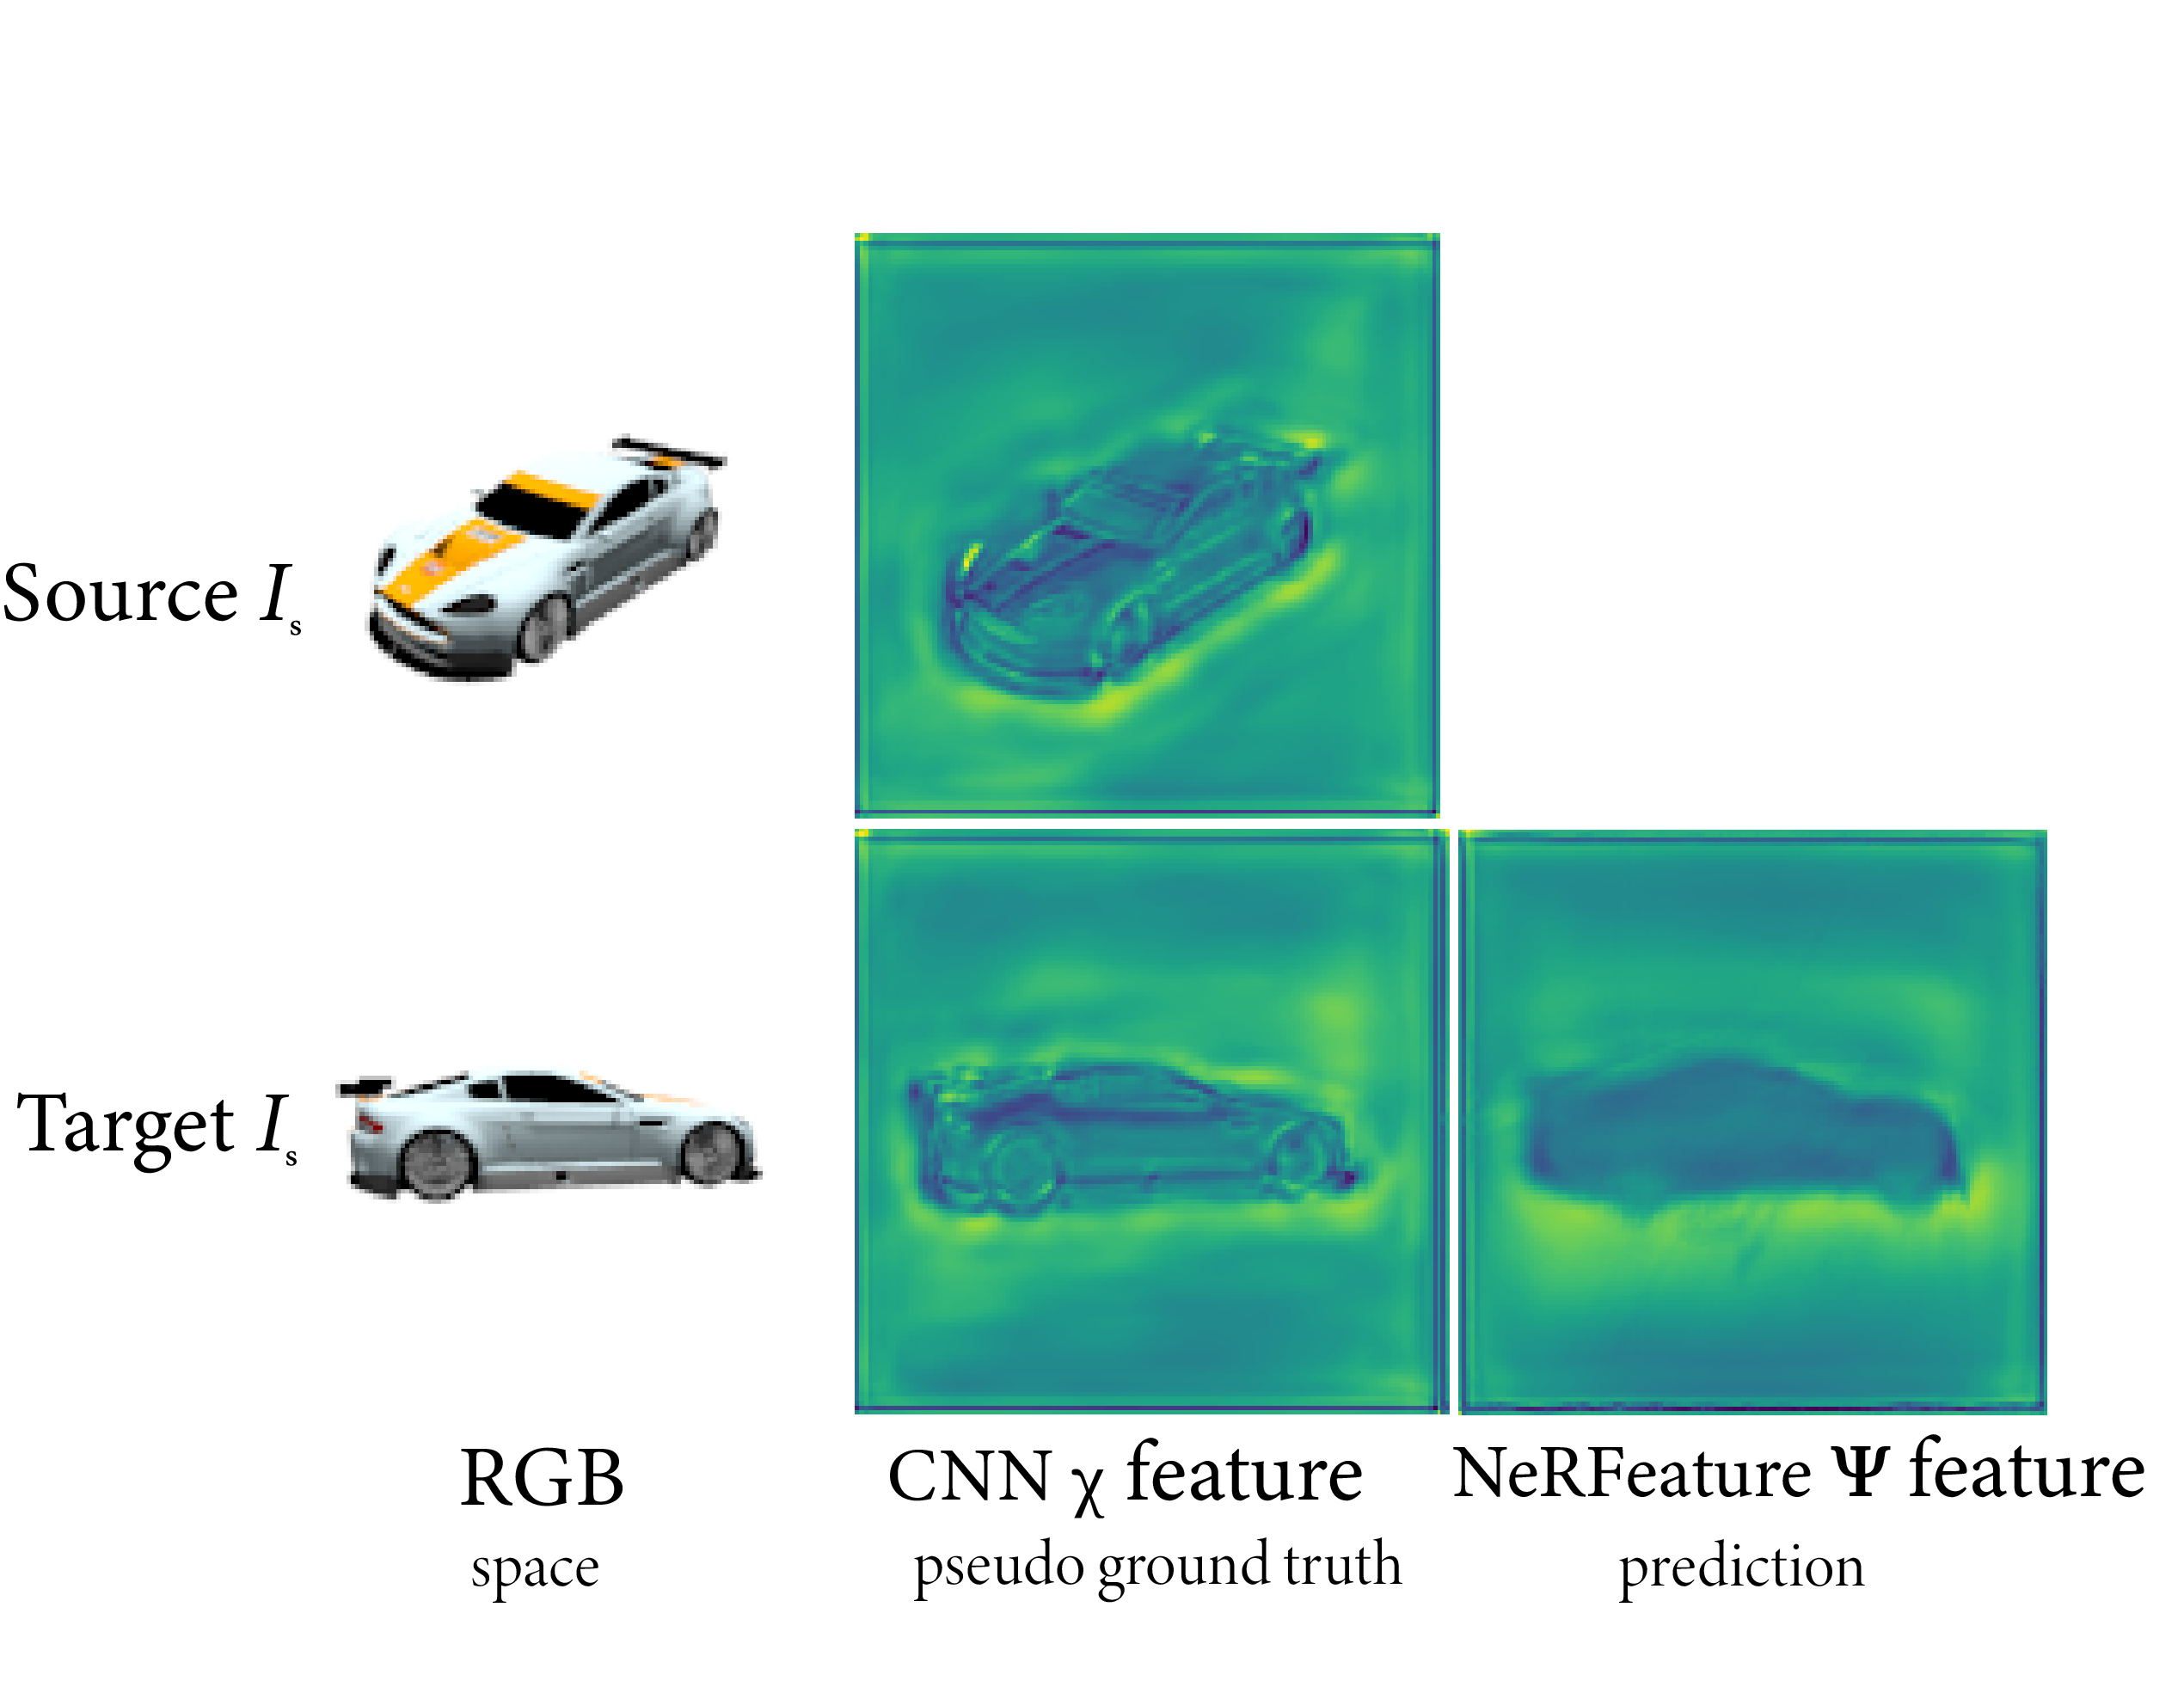
\includegraphics[width=.48\linewidth]{images/epinerf/nerfeature-main.png}} &
\bmvaHangBox{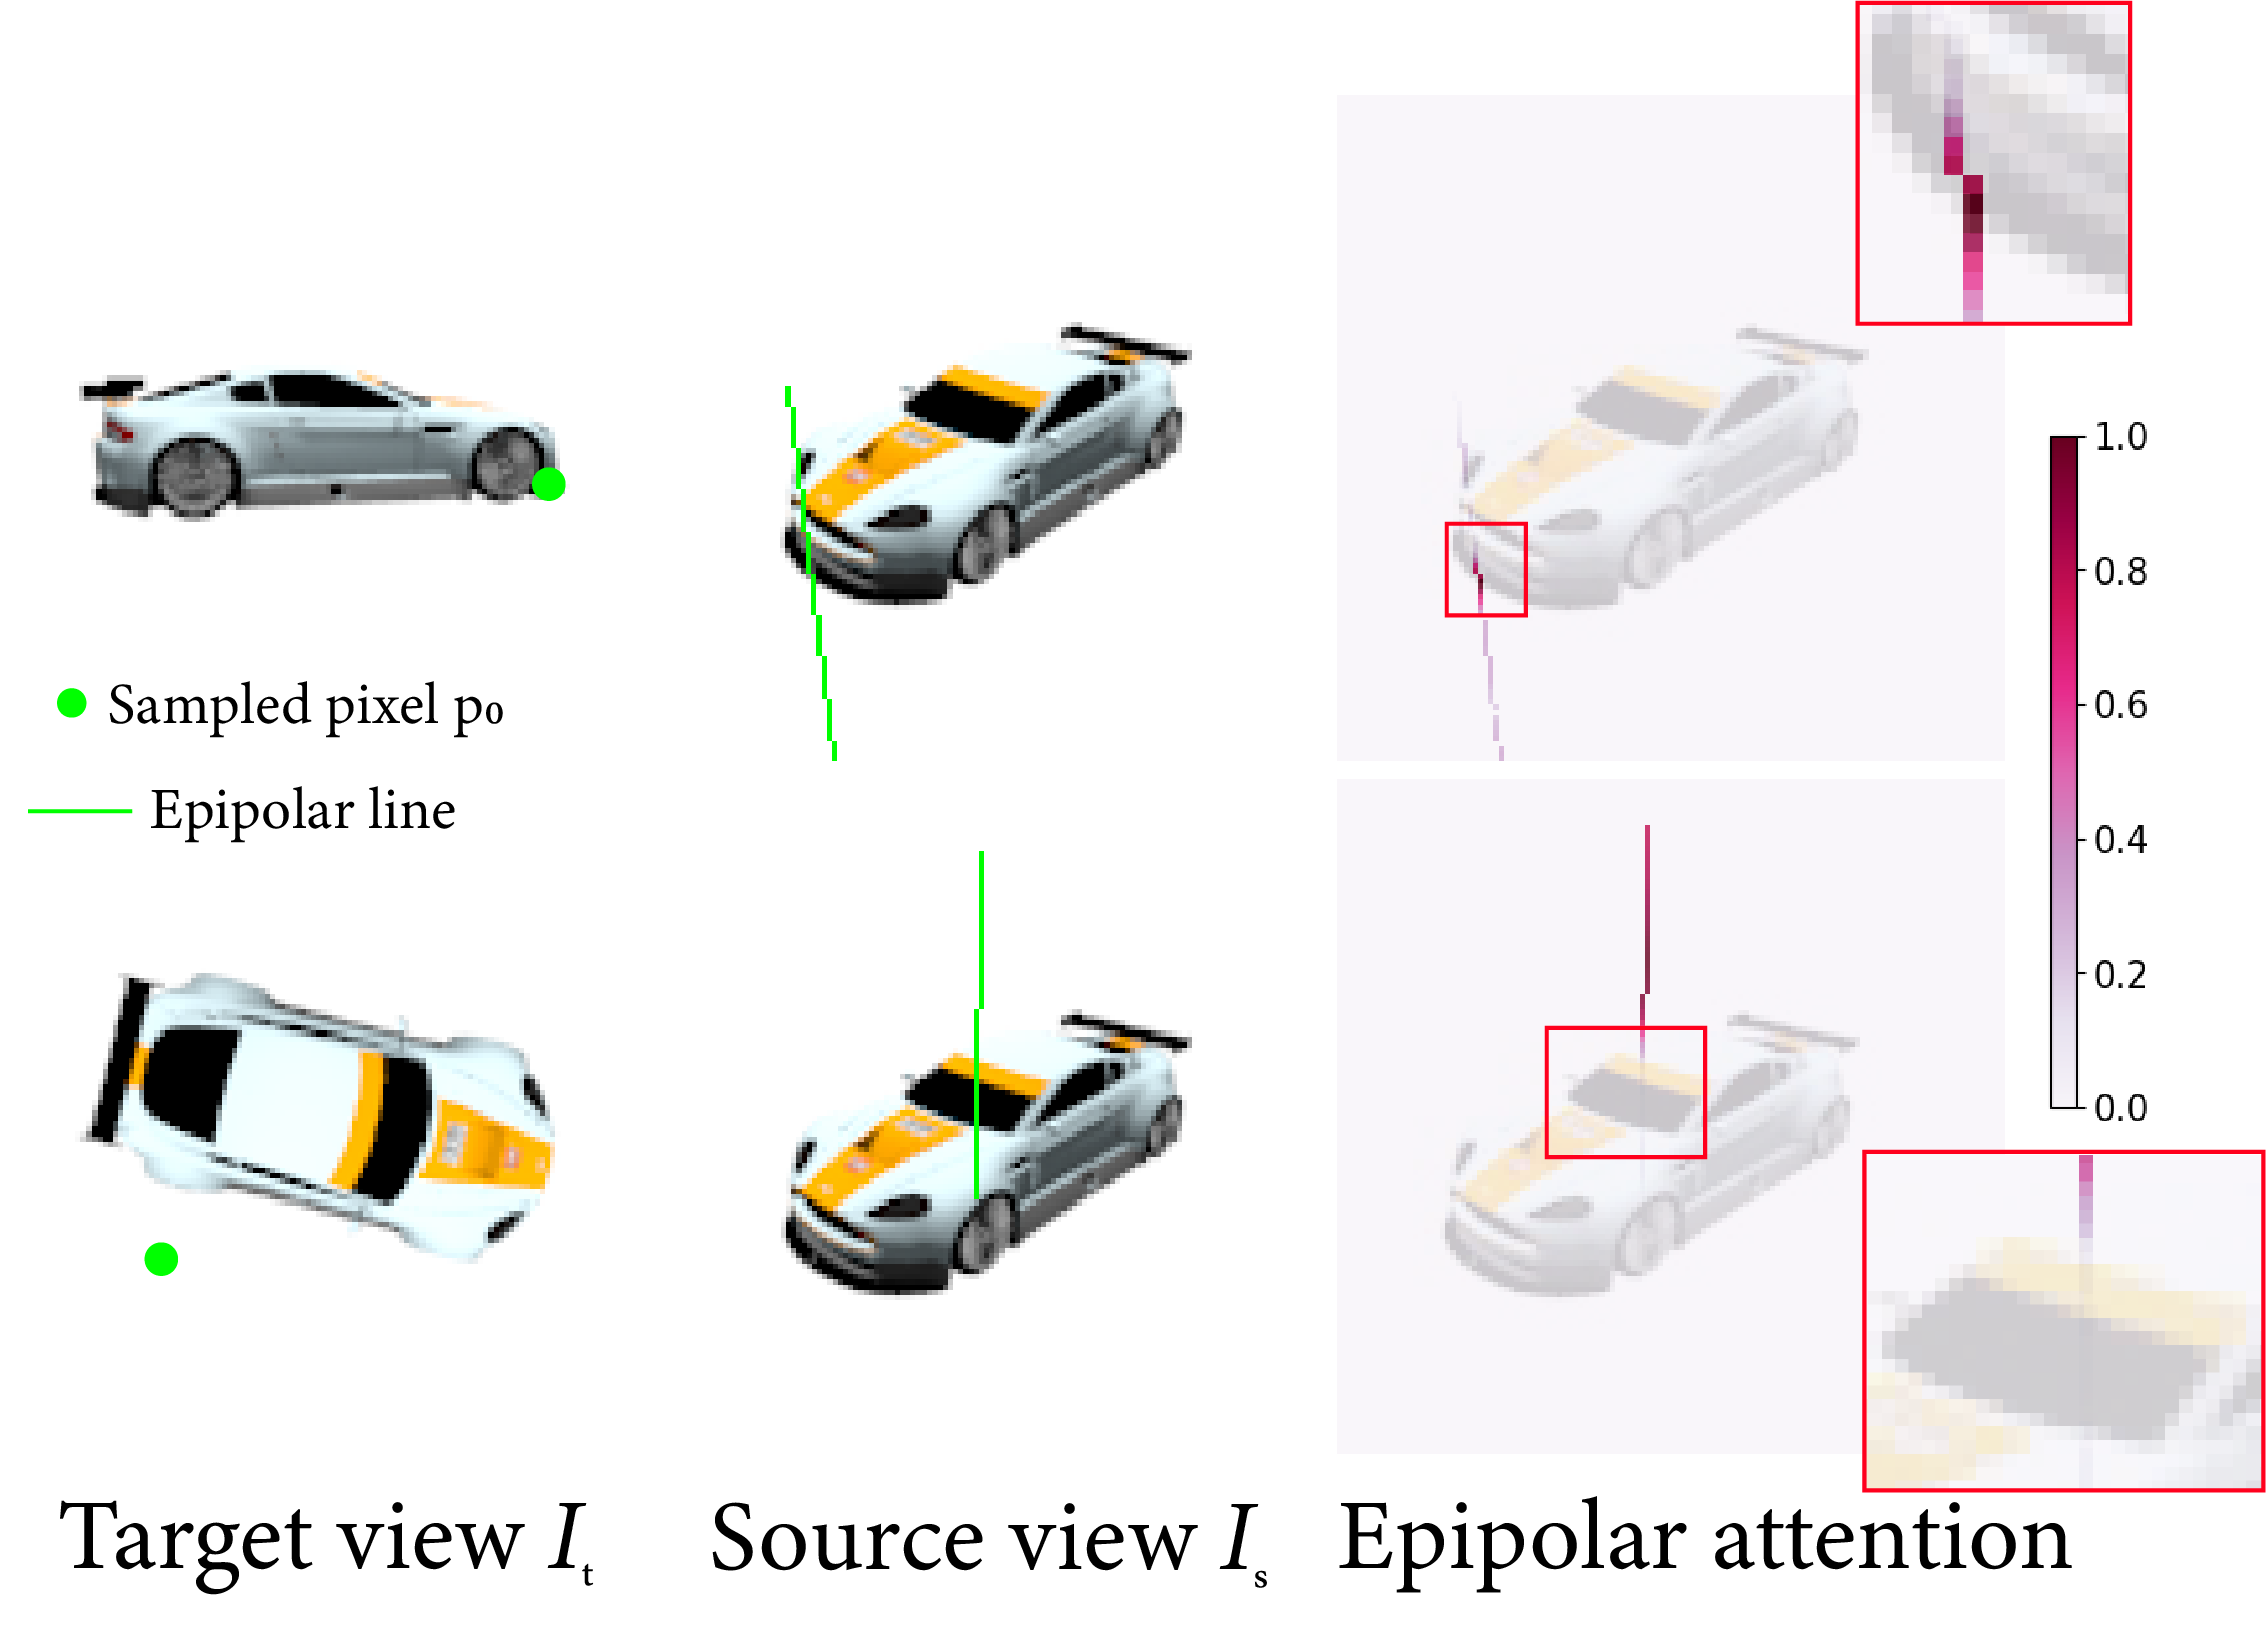
\includegraphics[width=.48\linewidth]{images/epinerf/attention_main.png}} \\
(a) & (b) \\
&

\end{tabular}
\caption{\textbf{Visual insights regarding NeRFeature and our epipolar attention mechanism.} (a) \textit{Pseudo} ground truth features are generated through our CNN encoder-decoder $\chi$. (b) Epipolar attention activation in two different scenarios.}
\label{fig:feat_and_att}
\end{center}
\end{figure}

\noindent \textbf{Epipolar attention.}
We depict on Figure \ref{fig:feat_and_att} (b) some visuals insights regarding our epipolar attention module. Considering a pixel $p_{0}$ sampled on the target view, the corresponding epipolar line is drawn in the source domain. As shown on the first row, if $p_{0}$ is sampled on the front right wheel, attention distribution along the epipolar line has its highest activation closed to the same regions, even though the wheel is not observed anymore in the source view domain. On the other hand, sampling $p_{0}$ on a background empty area (bottom row) leads in high attention scores along the epipolar line until car roof is crossed.  


\section{Conclusion}

In this paper, we propose a novel NeRF-based single-image NVS architecture. The NeRF architecture relies on an original \textit{local} and \textit{global} conditioning. Local since the CNN representation of the source image pixels is used as NeRF's input and global as the whole learnable NeRF's weights are obtained via an hypernetwork. The proposed method can be summarised as follow: 1) A first NeRF is learned to give access to high resolution source-aligned features ; 2) This set of features is distilled to a second radiance field, termed NeRFeature. It aims to predict high resolution target-aligned features. These two NeRFs and the CNN are joined to form the proposed EpiNeRF architecture; 3) In a final stage, EpiNeRF is fine-tuned. EpiNeRF main innovation lies on the epipolar constraint that is implemented in the RGB volume rendering via a lightweight feature-based attention mechanism. Theses contributions enables EpiNeRF to improved 3D points sampling and consequently achieve a more realistic final rendering result compared to current state-of-the-art methods. We demonstrated our claims on extensive experiments and ablation studies, and pushed towards a better integration of 3D priors through epipolar and symmetrical constraints within generalizable NeRF architectures. 
